%! Author = adrien koumgang tegantchouang
%! Date = 09/07/24

% Preamble
\documentclass[a4paper, 12pt]{report}
\usepackage[osf]{libertinus}
\pagestyle{plain}
\usepackage[top=2.5cm,bottom=2.5cm,left=4cm,right=2.5cm, centering]{geometry}
\linespread{1.5}
\usepackage[utf8]{inputenc} % codifica UTF-8
\usepackage{scrlayer-scrpage} % stili pagina per il frontespizio
\pagestyle{scrplain}
\usepackage{mathptmx} % font Times New Roman (simile)
\usepackage{graphicx, wrapfig}
\usepackage{lipsum}

\usepackage{url}
\usepackage{changepage}
\usepackage{multicol}
\usepackage{caption}
\usepackage{subcaption} % For the images' captions
\usepackage[linesnumbered,ruled,vlined]{algorithm2e}
\usepackage{amsmath} % For math symbols
\usepackage{amsthm} % Theorem styles
\usepackage{amssymb} % For special symbols % \mathbb and others
\usepackage{mathrsfs} % An alternative font for categories and sheaves.
\usepackage{cite} % For multiple citations
% \usepackage{caption}
% \usepackage{subcaption} % For the images' captions
\usepackage[section]{placeins} % To not break (sub)-images in two
\usepackage{booktabs}
\usepackage{float} % Always for images
\usepackage{soul} % For the \ul command, to use lists with less vertical spacing
\usepackage{enumerate} % For (i) list style
\usepackage{glossaries}
% \usepackage{minted}

\usepackage{blindtext}
\usepackage{hyperref}

%\usepackage{biblatex} % Imports biblatex package
%\addbibresource{mybibliography.bib} % Import the bibliography file

\usepackage{listings}
% \usepackage{listings-rust}
% \usepackage{rustlistings}
\usepackage{xcolor} % Optional: for colored code
\renewcommand{\lstlistingname}{Code}% Listing -> Codice\renewcommand{\lstlistingname}{Code}% Listing -> Codice

\usepackage[noend]{algpseudocode}
\algnewcommand\algorithmicforeach{\textbf{for each}}
\algdef{S}[FOR]{ForEach}[1]{\algorithmicforeach\ \#1 \algorithmicdo}

% \usepackage{color}
\usepackage{ragged2e}
\usepackage{algorithmicx}
% \usepackage{algorithm}
% \usepackage{algorithm2e}
\usepackage{program}
% \usepackage{listings-rust}
\usepackage{mathtools}



% \usepackage{xcolor}
\definecolor{codegreen}{rgb}{0,0.6,0}
\definecolor{codegray}{rgb}{0.5,0.5,0.5}
\definecolor{codemauve}{rgb}{0.4,0.,0.4}
% \definecolor{codepurple}{rgb}{0.5,0.5,0.5}
% \definecolor{backcolour}{rgb}{0.95,0.95,0.92}

% Define a custom color
\definecolor{backcolour}{rgb}{0.95,0.95,0.92}
\definecolor{codegreen}{rgb}{0,0.6,0}
\definecolor{codekeywork3}{rgb}{0.82,0.56,0.43}
% Define a custom style
\lstdefinestyle{cpp}{
    language = C++,
    backgroundcolor=\color{backcolour},   % choose the background color
    basicstyle=\footnotesize,        % the size of the fonts that are used for the code
    breakatwhitespace=false,         % sets if automatic breaks should only happen at whitespace
    breaklines=true,                 % sets automatic line breaking
    captionpos=b,                    % sets the caption-position to bottom
    commentstyle=\color{codegreen},    % comment style
% deletekeywords={...},            % if you want to delete keywords from the given language
% escapeinside={\%*}{*)},          % if you want to add LaTeX within your code
    extendedchars=true,              % lets you use non-ASCII characters; for 8-bits encodings only, does not work with UTF-8
    firstnumber=1000,                % start line enumeration with line 1000
    frame=single,                    % adds a frame around the code
    keepspaces=true,                 % keeps spaces in text, useful for keeping indentation of code (possibly needs columns=flexible)
    keywordstyle=\color{blue},       % keyword style
    keywordstyle=[2]\color{blue},       % keyword style
    keywordstyle=[3]\color{codekeywork3},       % keyword style
    language=Octave,                 % the language of the code
% morekeywords={*},            % if you want to add more keywords to the set
    morekeywords=[2]{*, class, private, public},            % if you want to add more keywords to the set
    morekeywords=[3]{*, unsigned, int, bool, vector, set, tuple},            % if you want to add more keywords to the set
    numbers=left,                    % where to put the line-numbers; possible values are (none, left, right)
    numbersep=5pt,                   % how far the line-numbers are from the code
    numberstyle=\tiny\color{codegray}, % the style that is used for the line-numbers
    rulecolor=\color{black},         % if not set, the frame-color may be changed on line-breaks within not-black text (e.g. comments (green here))
    showspaces=false,                % show spaces everywhere adding particular underscores; it overrides 'showstringspaces'
    showstringspaces=false,          % underline spaces within strings only
    showtabs=false,                  % show tabs within strings adding particular underscores
    stepnumber=1,                    % the step between two line-numbers. If it's 1, each line will be numbered
    stringstyle=\color{codemauve}, % string literal style
    tabsize=4, % sets default tabsize to 2 spaces
    alsoother={\<},
    alsoother={\>},
    morecomment=[l]{//},
    morecomment=[s]{/*}{*/}
}

\lstdefinestyle{rust}{
    language = Rust,
    backgroundcolor=\color{backcolour},   % choose the background color
    basicstyle=\footnotesize,        % the size of the fonts that are used for the code
    breakatwhitespace=false,         % sets if automatic breaks should only happen at whitespace
    breaklines=true,                 % sets automatic line breaking
    captionpos=b,                    % sets the caption-position to bottom
    commentstyle=\color{codegreen},    % comment style
% deletekeywords={...},            % if you want to delete keywords from the given language
% escapeinside={\%*}{*)},          % if you want to add LaTeX within your code
    extendedchars=true,              % lets you use non-ASCII characters; for 8-bits encodings only, does not work with UTF-8
    firstnumber=1000,                % start line enumeration with line 1000
    frame=single,                    % adds a frame around the code
    keepspaces=true,                 % keeps spaces in text, useful for keeping indentation of code (possibly needs columns=flexible)
    keywordstyle=\color{blue},       % keyword style
    keywordstyle=[2]\color{blue},       % keyword style
    keywordstyle=[3]\color{codekeywork3},       % keyword style
    language=Octave,                 % the language of the code
% morekeywords={*},            % if you want to add more keywords to the set
    morekeywords=[2]{*, pub, struct, fn, impl, let, match, as},            % if you want to add more keywords to the set
    morekeywords=[3]{*, bool, char, f32, f64, i8, i16, i32, i64, isize, str, u8, u16, u32, u64, unit, usize, i128, u128},            % if you want to add more keywords to the set
    numbers=left,                    % where to put the line-numbers; possible values are (none, left, right)
    numbersep=5pt,                   % how far the line-numbers are from the code
    numberstyle=\tiny\color{codegray}, % the style that is used for the line-numbers
    rulecolor=\color{black},         % if not set, the frame-color may be changed on line-breaks within not-black text (e.g. comments (green here))
    showspaces=false,                % show spaces everywhere adding particular underscores; it overrides 'showstringspaces'
    showstringspaces=false,          % underline spaces within strings only
    showtabs=false,                  % show tabs within strings adding particular underscores
    stepnumber=1,                    % the step between two line-numbers. If it's 1, each line will be numbered
    stringstyle=\color{codemauve}, % string literal style
    tabsize=4, % sets default tabsize to 2 spaces
    alsoother={\<},
    alsoother={\>},
    morecomment=[l]{//},
    morecomment=[s]{/*}{*/}
}

\lstdefinestyle{python}{
    language=Python,                    % Set language to Python
    basicstyle=\ttfamily\footnotesize,   % Basic font style for the code
    keywordstyle=\color{blue}\bfseries,  % Style for keywords
    stringstyle=\color{red},             % Style for strings
    commentstyle=\color{gray}\itshape,   % Style for comments
    numberstyle=\tiny\color{gray},       % Style for line numbers
    numbers=left,                        % Show line numbers on the left
    stepnumber=1,                        % Line numbers every 1 line
    numbersep=8pt,                       % Space between line numbers and code
    tabsize=4,                           % Width of a tab
    showspaces=false,                    % Don't show spaces
    showstringspaces=false,              % Don't show spaces in strings
    showtabs=false,                      % Don't show tab characters
    frame=single,                        % Add a frame around the code
    rulecolor=\color{black},             % Frame color
    captionpos=b,                        % Position of caption (bottom)
    breaklines=true,                     % Automatically break long lines
    breakatwhitespace=true,              % Allow breaking at whitespace
    backgroundcolor=\color{white},       % Set background color
    morekeywords={self, None, True, False}, % Additional Python-specific keywords
    % escapeinside={(*@}{@*)},             % Escape inside code
    literate={\<}{{\textless}}1 {\>}{{\textgreater}}1, % Handle < and > symbols
}

% \lstdefinestyle{mystyle}{
%    backgroundcolor=\color{backcolour},
%    commentstyle=\color{codegreen},
%    keywordstyle=\color{magenta},
%    numberstyle=\tiny\color{codegray},
%    stringstyle=\color{codepurple},
%    basicstyle=\ttfamily\footnotesize,
%    breakatwhitespace=false,
%    breaklines=true,
%    captionpos=b,
%    keepspaces=true,
%    numbers=left,
%    numbersep=5pt,
%    showspaces=false,
%    showstringspaces=false,
%    showtabs=false,
%    tabsize=4
% }


\newtheorem{mydef}{Definition}
\newtheorem{mytheo}{Theorem}
\newtheorem{mylem}{Lemma}
\newtheorem{mypro}{Property}
\newtheorem{myex}{Example}
\newtheorem{mycor}{Corollary}
\newtheorem{myproof}{Proof idea}
\newtheorem{mypc}{Pseudocode}



\begin{document}
    \begin{titlepage} %crea l'enviroment
\begin{figure}[t] %inserisce le figure
    \centering
\includegraphics[width=0.80\textwidth]{marchio_unipi_pant541}\label{fig:figure-first-page}
\end{figure}

\vspace{20mm}

\begin{Large}
 \begin{center}
	\textbf{Dipartimento di Informatica\\ Corso di Laurea Triennale in Informatica\\}
	\vspace{2cm}
    {\LARGE{TESI DI LAUREA}}\\
	\vspace{2cm}
	{\Large{Algorithmic aspects of Modular Decomposition Implementation}}
\end{center}
\end{Large}

\vspace{15mm}

%minipage divide la pagina in due sezioni settabili
\begin{minipage}[t]{0.47\textwidth}
	{\large{\textbf{Relatore esterno:\\ Prof. Frédéric Peschanshi \\ Prof. Antoine Genitrini}}}

	\vspace{0.5cm}

	{\large{\textbf{Relatore interno: \\ Prof. Andrea Corradini}}}
\end{minipage}
\hfill
\begin{minipage}[t]{0.47\textwidth}\raggedleft
	{\large{\textbf{Candidato: \\ Adrien Koumgang Tegantchouang}}}
\end{minipage}

\vspace{20mm}

\centering{\large{\textbf ANNO ACCADEMICO 2023/2024 }}

\end{titlepage}


    \tableofcontents

% \listoffigures


    \thispagestyle{empty}

    \clearpage
    \setcounter{page}{1}


% Preambule (A Survey on Algorithmic Aspects of Modular Decomposition)
% \include{chapters/chapter_00}


% Introduction
    %! Author = adrienkoumgangtegantchouang
%! Date = 09/07/24

\chapter{Introduction}\label{ch:introduction}


\section{Overview}\label{sec:overview}

The field of graph theory is a cornerstone of computer science and discrete mathematics, offering a rich framework for modeling and analyzing complex networks.
Among the various techniques and algorithms developed within this domain, modular decomposition stands out due to its ability to simplify and break down graphs into smaller, more manageable components called modules.
This decomposition is pivotal for solving numerous combinatorial optimization problems, including those found in bioinformatics, social network analysis, and communication networks.

This thesis aims to delve into the modular decomposition of graphs, focusing on its theoretical foundations, algorithmic implementations, and practical performance evaluations.
By building upon the work of Eleni Pistiloglou, who explored the modular decomposition of 2-structures, this research seeks to extend her findings and improve upon them through the implementation of the modular decomposition algorithm in Rust, a programming language known for its performance and safety features.


\section{Objectives}\label{sec:objectives}

The main objectives of this thesis are as follows:

\begin{itemize}
    \item \textbf{Understanding Modular Decomposition:} To comprehensively understand the concept of modular decomposition, its definitions, properties, and applications in graph theory and beyond.
    \item \textbf{Extending Previous Work:} To build upon Eleni Pistiloglou's work on 2-structures, enhancing the understanding of modular decomposition in this context.
    \item \textbf{Algorithm Implementation:} To implement the modular decomposition algorithm in Rust and in C++.
    \item \textbf{Performance Comparison:} To rigorously evaluate and compare the performance of the Rust implementation against Python and SageMath, particularly focusing on execution time and scalability with different graph sizes.
\end{itemize}


\section{Structure of the Thesis}\label{sec:structure-of-the-thesis}

This thesis is structured to guide the reader through the comprehensive study and findings of this research.
The chapters are organized as follows:

\begin{itemize}
    \item \textbf{Chapter \ref{ch:modular-decomposition}: Modular Decomposition}: This chapter delves into the theoretical aspects of modular decomposition, defining key concepts such as modules, maximal modular partitions, and the application of these concepts to oriented graphs and 2-structures.
    \item \textbf{Chapter \ref{ch:implementation-of-modular-decomposition}: Implementation of modular decomposition}: This chapter presents the modular decomposition algorithm, detailing its steps, pseudocode, and a comprehensive example to illustrate the algorithm's application.
    \item \textbf{Chapter \ref{ch:previous-work-implementation-in-sagemath-and-python}: Previous Work: Implementation in SageMath and Python}: This chapter presents the work previously done, including the SageMath and Python implementations, with a particular focus on the Python version and its performance against SageMath.
    \item \textbf{Chapter \ref{ch:implementation-in-rust-and-cpp}: Implementation in Rust and C++}: This chapter discusses the implementation process in C++ and Rust, highlighting the transition from C++ to Rust and comparing the Rust implementation with the existing Python version.
    \item \textbf{Chapter \ref{ch:benchmarking}: Benchmarking}: This chapter outlines the methodology used for performance testing, presents the results, and provides an in-depth analysis of the performance of the different implementations.
\end{itemize}



% modular decomposition
    %! Author = adrienkoumgangtegantchouang
%! Date = 09/07/24

\chapter{Modular Decomposition}\label{ch:modular-decomposition}


Modular decomposition is a fundamental concept in graph theory and combinatorial optimization that simplifies the analysis and processing of graphs.
By breaking down a graph into smaller, more manageable subgraphs known as modules, modular decomposition enables more efficient algorithms for various graph-related problems.
This chapter provides an overview of modular decomposition, including its definitions, properties, applications, and examples.


\section{Definition of graph}\label{sec:definition-of-graph}

A graph is a mathematical structure used to model pairwise relations between objects. \cite{GT1,GT2}

\begin{mydef}
    A graph $G$ is defined as an ordered pair $G = (V, E)$, where
    \begin{itemize}
        \item $V$ is a finite set of vertices (or nodes).
        \item $E$ is a set of edges (or arcs), where each edge is a pair of vertices.
    \end{itemize}
\end{mydef}

Graphs can be broadly categorized into two types based on the nature of their edges: undirected graphs and directed graphs.

\subsection*{Undirected Graph}\label{subsec:undirected-graph}

An undirected graph is a type of graph in which the edges have no orientation.
The edges simply connect two vertices and do not have a direction associated with them.

An undirected graph is a graph $G = (V, E)$ where $E \subseteq P_2(V)$, i.e., $E$ is a set of subsets of nodes of cardinality 2.
Therefore, each edge $\{u, v\}$ is an unordered pair of vertices.

In undirected graphs, the edge $\{u, v\}$ is identical to the edge $\{v, u\}$, implying that the connection is bidirectional.

Example~\cite{mdwikipedia}: an undirected graph $G$ with vertices $V = \{v1, v2, v3, v4, v5, v6, v7, v8, v9, v10, v11\}$ and edges \\
$E= \{\{v1, v2\}, \{v1, v3\}, \{v1, v4\}\}$
$\cup \; \{\{v2, v4\}, \{v2, v5\}, \{v2, v6\}, \{v2, v7\}\}$ \\
$\cup \; \{\{v3, v4\}, \{v3, v5\}, \{v3, v6\}, \{v3, v7\}\}$
$\cup \; \{\{v4, v5\}, \{v4, v6\}, \{v4, v7\}\}$
$\cup \; \{\{v5, v6\}, \{v5, v7\}\}$
$\cup \; \{\{v6, v8\}, \{v6, v9\}, \{v6, v10\}, \{v6, v11\}\}$
$\cup \; \{\{v7, v8\}, \{v7, v9\}, \{v7, v10\}, \{v7, v11\}\}$
$\cup \; \{\{v8, v9\}, \{v8, v10\}, \{v8, v11\}\}$
$\cup \; \{\{v9, v10\}, \{v9, v11\}\}$


\begin{figure}[!h]
    \centering
    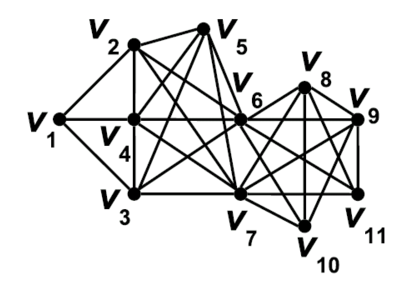
\includegraphics[width=0.40\textwidth]{images/graphs/undirected_graph_wikipedia}
    \caption{Example of Undirected Graph}
    \label{fig:example-undirected-graph}
\end{figure}

Undirected graphs are commonly used in scenarios where the relationships are mutual, such as social networks where friendships are bidirectional.

\subsection*{Directed Graph}\label{subsec:directed-graph}

A directed graph, or digraph, is a type of graph in which the edges have a direction, indicating a one-way relationship between the vertices.

A directed graph is a graph $G = (V, E)$ where $E \subseteq V \times V$, i.e., $E$ is a binary relation on $V$.
Therefore, each edge $(v, w)$ is an ordered pair of vertices.

In directed graphs, the edge $(u, v)$ is not identical to the edge $(v, u)$, implying that the connection is unidirectional.

Example: a directed graph $G$ with vertices $V = \{1, 2, 3, 4, 5, 6, 7, 8\}$ and edges \\
$E = \{(1, 2), (1, 3)\}$
$\cup \; \{(2, 3)\}$
$\cup \; \{(4 , 1), (4, 2), (4, 3), (4, 6)\}$
$\cup \; \{(5 , 1), (5, 2), (5, 3), (5, 6)\}$
$\cup \; \{(6, 4), (6, 5), (6, 7), (6, 8)\}$
$\cup \; \{(7, 8)\}$
$\cup \; \{(8, 7)\}$

\begin{figure}[!h]
    \centering
    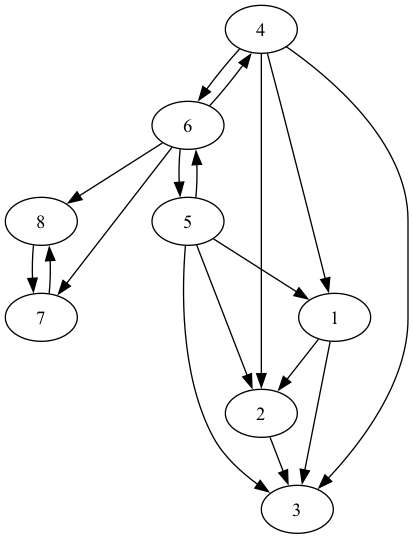
\includegraphics[width=0.40\textwidth]{images/graphs/digraph_ex1_without_label}
    \caption{Example of Directed Graph}
    \label{fig:example-directed-graph}
\end{figure}

Directed graphs are used where relationships have a direction, such as web page links (where one page links to another) or task scheduling (where one task must precede another).


\section{Definition of Modular Decomposition}\label{sec:definition-of-modular-decomposition}

\subsection*{Module}\label{subsec:module}

Modular decomposition involves partitioning the vertex set $V$ into subsets, or modules, that have specific properties relative to the rest of the graph.

A \textbf{module}~\cite{mdwikipedia} of a graph is a generalization of a connected component~\cite{componentwikipedia}.
In graph theory, a \textbf{component} of an undirected graph is a connected subgraph that is not part of any larger connected subgraph.
The components of any graph partition its vertices into disjoint sets, and are the induced subgraphs of those sets.
A graph that is itself connected has exactly one component, consisting of the whole graph.
Components are sometimes called \textbf{connected components}.

\begin{figure}[!h]
    \centering
    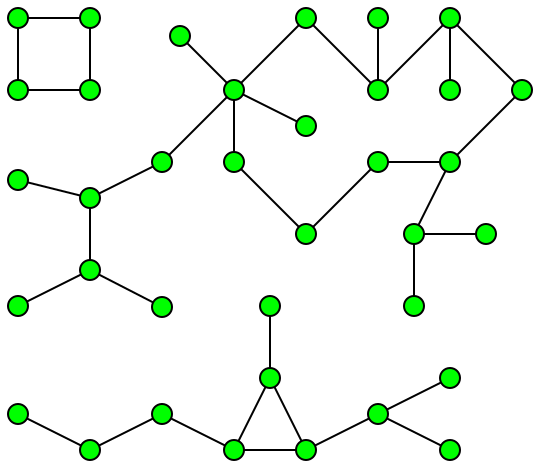
\includegraphics[width=0.40\textwidth]{images/graphs/Pseudoforest}
    \caption{Example of Modules (A graph with three components) \cite{componentwikipedia}}
    \label{fig:example-modules}
\end{figure}

A connected component has the property that it is a set $M$ of vertices such that every member of $M$ is a non-neighbor of every not vertex in $M$.
(It is a union of connected components if and only if it has this property.)
More generally, $M$ is a module if, for each vertex $m \notin M$, either every member of $M$ is a non-neighbor of $m$ or every member of $M$ is a neighbor of $m$.

Equivalently, $M$ is a module if all members of $M$ have the same set of neighbors among vertices not in $M$.

Another definition of components involves the equivalence classes of an equivalence relation defined on the graph's vertices.
In an undirected graph, a vertex $v$ is reachable from a vertex $u$, if there is a path from $u$ to $v$, or equivalently a walk (a path allowing repeated vertices and edges).
Reachability is an equivalence relation, since:
\begin{itemize}
    \item It is \textbf{reflexive}: There is a trivial path of length zero from any vertex to itself.
    \item It is \textbf{symmetric}: If there is a path from $u$ to $v$, the same edges in the reserve order from a path from $v$ to $u$.
    \item It is \textbf{transitive}: If there is a path from $u$ to $v$ and a path from $v$ to $w$, the two paths may be concatenated together to form a walk from $u$ to $w$.
\end{itemize}

\begin{mydef}
(Module)
    A module $M \subseteq V$ of a graph $G$ is a subset of vertices such that every vertex in $M$ has the same set of neighbors outside $M$.
    Formally, for any $u, v \in M$ and any $w \in V - M$, $w$ is adjacent to $u$ if and only if $w$ is adjacent to $v$.
\end{mydef}

This definition ensures that within a module, the vertices are indistinguishable based on their connections to the rest of the graph.
Modules can vary in size and structure, from single vertices to large subgraphs encompassing a significant portion of the original graph.

Contrary to the connected components, the modules of a graph are the same as the modules of its complement, and modules can be nested: one module can be a proper subset of another.
Note that the set $V$ of vertices of a graph is a module, as are its one-element subsets and the empty set; these are called the \textbf{trivial modules}.
A graph may or may not have other modules.
A graph is called \textbf{prime} if all of its modules are trivial.

In the mathematical field of graph theory, the complement~\cite{complementgraphwikipedia} or inverse of a graph $G$ is a graph $H$ on the same vertices such that two distinct vertices of $H$ are adjacent if and only if they are not adjacent in $G$.
That is, to generate the complement of a graph, one fills in all the missing edges required to form a complete graph, and removes all the edges that were previously there.
The complement is not the set complement of the graph; only the edges are complemented.

\begin{figure}[!h]
    \centering
    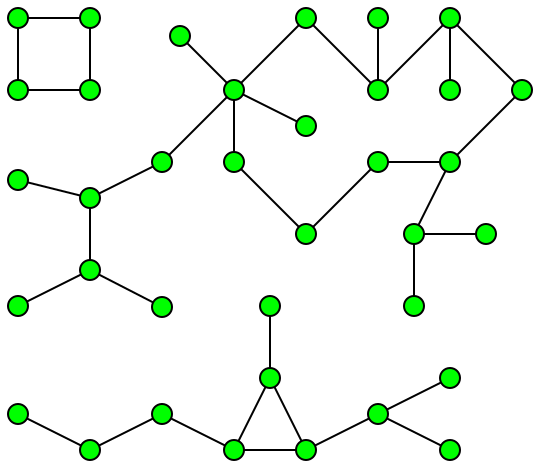
\includegraphics[width=0.40\textwidth]{images/graphs/Pseudoforest}
    \caption{The Petersen graph (on the left) and its complement graph (on the right) \cite{complementgraphwikipedia}}
    \label{fig:the}
\end{figure}


\subsection*{Modular Partition}\label{subsec:modular-partition}

In graph theory, partitioning a graph into meaningful substructures is a common strategy for simplifying complex problems.
A modular partition specifically refers to dividing the vertices of a graph into disjoint subsets, known as modules, where each subset satisfies certain uniformity conditions relative to the rest of the graph.
This concept is crucial for understanding the deeper hierarchical structure of graphs and forms the foundation for various graph decomposition techniques.

\begin{mydef}
    A modular partition of a graph $G = (V, E)$ is a partition of the vertex set $V$ into disjoint subsets $M_1$, $M_2$, \ldots, $M_k$ such that each subset $M_i$ (for $i = 1, 2, \ldots, k$) is a module.
\end{mydef}

\subsubsection*{Properties of Modular Partitions}

Modular partitions possess several important properties that make them useful for graph analysis:

\begin{enumerate}
    \item \textbf{Uniform Neighborhood:} Within a module, all vertices share the same neighbors outside the module.
    This property allows for simplification of the graph by treating the entire module as a single unit when considering its external connections.
    \item \textbf{Independence from Internal Structure:} The internal structure of a module does not affect its status as a module.
    This means that the relationships between vertices within a module are irrelevant to the modular partitioning, focusing solely on external connections.
    \item \textbf{Hierarchical Organization:} Modular partitions naturally lead to a hierarchical organization of the graph.
    By recursively partitioning modules into smaller modules, one can build a modular decomposition tree that captures the multi-level structure of the graph.
\end{enumerate}

To illustrate the concept of modular partitions, consider the following examples:

\begin{myex}[Simple Undirected Graph]
    Consider an undirected graph $G$ from Figure~\ref{fig:example-undirected-graph}.

    In this graph, the sets $\{v2, v3, v4\}$ and $\{v6, v7\}$ each form modules.
    The non trivial modules are: $\{2, 3\}, \{2, 3, 4\}, \{6, 7\}, \{10, 11\}, \{8, 9, 10, 11\}$.
    Possible modular partition are:
    \begin{itemize}
        \item $\{\{v1\}, \{v2, v3, v4\}, \{v5\}, \{v6, v7\}, \{v8, v9, v10, v11\}\}$
        \item $\{\{v1\}, \{v2, v3\}, \{v4\}, \{v5\}, \{v6, v7\}, \{v8\}, \{v9\}, \{v10, v11\}\}$
    \end{itemize}
    The last one is the maximal modular partition.
\end{myex}

\begin{myex}[Directed Graph]
    Consider a directed graph $G$ from Figure~\ref{fig:example-directed-graph}.

    In this graph, the sets $\{2, 3\}$, $\{4, 5\}$, and $\{6, 7, 8\}$ each form modules.
    Thus, a possible modular partition of $G$ is $\{\{1\}, \{2, 3\}, \{4, 5\}, \{6, 7, 8\}\}$.
\end{myex}

\subsection*{Maximal Modular Partition}\label{subsec:maximal-modular-partition}

The maximal modular partition of a graph is unique and consists of the largest possible prime modules.
Prime modules are those that cannot be further decomposed into smaller non-trivial modules.

\begin{mydef}
(Maximal modular partition)
    The maximal modular partition of a graph $G$ is the partition consisting of the largest prime modules.
    This partition is unique and is often represented as a tree, known as the modular decomposition tree, where each node corresponds to a module, and the leaves are the individual vertices of the graph.
\end{mydef}


\section{Application to 2-Structures}\label{sec:application-to-2-structures}

Modular decomposition extends naturally to 2-structures, which are complete directed graphs with arcs colored from a set of $k$ colors.
The additional complexity of orientation and coloring requires modified definitions and algorithms for modular decomposition.

A 2-structure is a generalization of a graph where edges (or arcs) between vertices are assigned different colors or types, capturing more complex relationships between vertices.
This concept is particularly useful in scenarios where the simple binary relationship (edge or no edge) in standard graphs is insufficient to model the nuances of the interactions between entitites.

\begin{mydef}
    A 2-structure $G$ is defined as a pair $G = (V, A)$, where
    \begin{itemize}
        \item $V$ is a finite set of vertices.
        \item $A$ is a set of arcs, where each arc is a triple $(u, v, c)$ consisting of an ordered pair of vertices $u$ and $v$, and a color or type $c$.
    \end{itemize}
\end{mydef}

In a 2-structure, the arc $(u, v, c)$ indicates a directed relationship from vertex $u$ to vertex $v$ with a specific color or type $c$.

thus follows the properties of the 2-structures:

\begin{enumerate}
    \item \textbf{Directed and Colored Arcs:} Unlike standard graphs where edges are typically uncolored, 2-structures have arcs that are both directed and colored.
    This allows for a richer representation of relationships.
    \item \textbf{Complex Relationships:} The use of colors or types for arcs allows 2-structures to model complex relationships between vertices, where the nature of the relationship is significant.
    \item \textbf{Generalization:} 2-structures generalize both undirected and directed graphs.
    An undirected graph can be seen as a 2-structure where each edge is represented by two directed arcs of the same color (one in each direction).
    A directed graph is a 2-structure where arcs are colored uniformly.
\end{enumerate}

\begin{myex}[2-Structure]
    Consider a 2-structure $G$ with vertices $V = \{u, v, w, x\}$ and arcs $A = \{(u, v, 1), (u, w, 1), (v, w, 2), (w, x, 1)\}$, where the third element in each triple represents the color of the arc.

    \begin{figure}[!h]
        \centering
        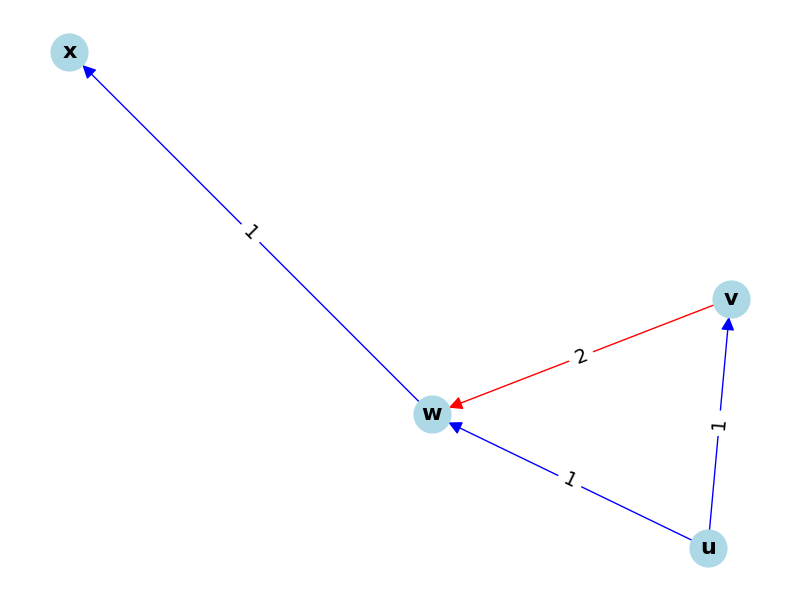
\includegraphics[width=0.40\textwidth]{images/graphs/2_structure_graph_example}
        \caption{Example of 2 Structure Graph}
        \label{fig:2-structure-graph-example-simple}
    \end{figure}

    In this 2-structure:
    \begin{itemize}
        \item The set of vertices $V$ is $\{u, v, w, x\}$
        \item The set of arcs $A$ includes:
        \begin{itemize}
            \item $(u, v, 1)$ indicating a type-1 arc from $u$ to $v$.
            \item $(u, w, 1)$ indicating a type-1 arc from $u$ to $w$.
            \item $(v, w, 2)$ indicating a type-2 arc from $v$ to $w$.
            \item $(w, x, 1)$ indicating a type-1 arc from $w$ to $x$.
        \end{itemize}
    \end{itemize}
\end{myex}

Another example of 2-structure from directed graph from Figure~\ref{fig:example-directed-graph} is:
\begin{myex}[Another 2-structure]
    \begin{figure}[!h]
        \centering
        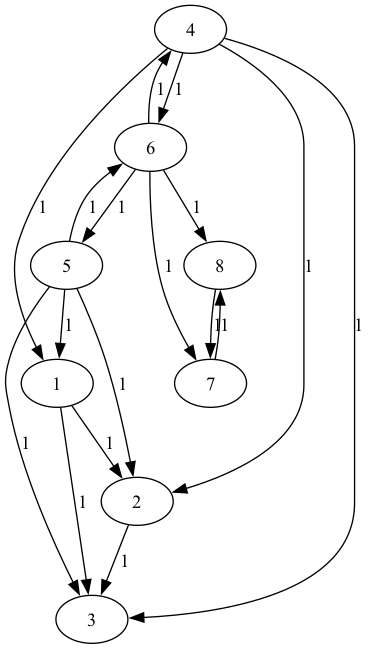
\includegraphics[width=0.30\textwidth]{images/graphs/digraph_ex1}
        \caption{Example of 2 Structure Graph}
        \label{fig:2-structure-graph-example}
    \end{figure}
\end{myex}


The definition of modules in 2-structures incorporates both the direction and color of arcs.

\begin{mydef}
    A module $M$ in a 2-structure $G$ is a subset of vertices such that for any $u, v \in M$ and any $w \in V - M$, the arcs $(w, u, c)$ and $(w, v, c)$ have the same color and direction, and the arcs $(u, w, c)$ and $(v, w, c)$ have the same color and direction.
\end{mydef}


\section{Examples of Modular Decomposition}\label{sec:examples-of-modular-decomposition}

To illustrate the concept of modular decomposition, consider the following examples.

% \subsection*{Example 1: Simple Undirected Graph}\label{subsec:example-1:-simple-undirected-graph}

\begin{myex}[Simple Undirected Graph]
    \label{ex:simple-undirected-graph}

Consider an undirected graph $G$ from Figure~\ref{fig:example-undirected-graph}, the modules of this graph are:

\begin{itemize}
    \item $\{v1\}$.
    \item $\{v2, v3, v4\}$.
    \item $\{v5\}$.
    \item $\{v6, v7\}$.
    \item $\{v8, v9, v10, v11\}$.
\end{itemize}

\begin{figure}[!h]
    \centering
    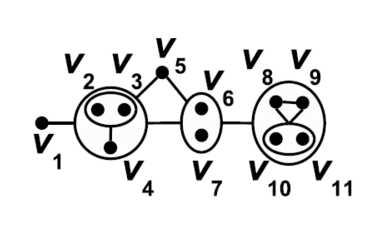
\includegraphics[width=0.40\textwidth]{images/graphs/undirected_graph_wikipedia_module}
    \caption{Example of Module for Simple Undirected Graph}
    \label{fig:example-undirected-graph-module}
\end{figure}

The maximal modular partition of $G$ is $\{\{v1\}, \{v2, v3\}, \{v4\}, \{v5\}, \{v6, v7\}, \{v8\}, \{v9\}, \{v10, v11\}\}$.
\end{myex}

\begin{myex}[Directed Graph (2-structure)]
    Consider a directed graph $G$ from Figure~\ref{fig:2-structure-graph-example}.

    The modules of this graph are $\{2, 3\}$, $\{4, 5\}$, $\{6\}$ and $\{7, 8\}$

    The maximal modular partition of $G$ is $\{\{1\}, \{2, 3\}, \{4, 5\}, \{6\}, \{7, 8\}\}$.
\end{myex}


\section{Modular Decomposition Tree}\label{sec:modular-decomposition-tree}

The modular decomposition tree represents the hierarchical structure of modules within a graph.
Each node in the tree corresponds to a module, and the leaves are the individual vertices of the graph.
The root node represents the entire graph.

\subsection*{Construction of the Tree}\label{subsec:construction-of-the-tree}

The modular decomposition tree is constructed as follows:

\begin{itemize}
    \item Identify the maximal modular partition of the graph.
    \item Represent each module as a node in the tree.
    \item Recursively apply the modular decomposition to each module, treating it as a subgraph.
    \item Connect the nodes to reflect the hierarchical structure of the modules.
\end{itemize}


\begin{Example}
    Consider the graph $G$ from Figure~\ref{fig:example-undirected-graph} with maximal modular partition \\ $\{\{v1\}, \{v2, v3, v4\}, \{v5\}, \{v6, v7\}, \{v8, v9, v10, v11\}\}$ (Figure~\ref{fig:example-undirected-graph-module}).
    The modular decomposition tree is constructed as follows:

    \begin{figure}[!h]
        \centering
        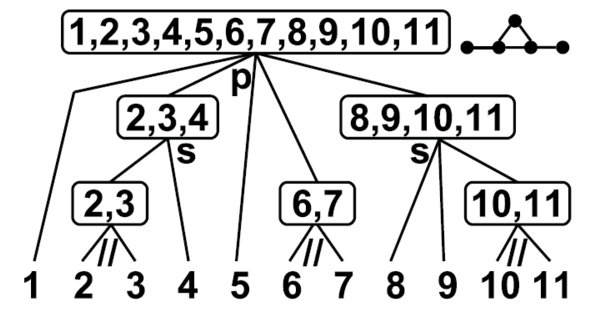
\includegraphics[width=0.40\textwidth]{images/graphs/undirected_graph_wikipedia_modular_decomposition}
        \caption{Example of Result of Modular Decomposition Tree}
        \label{fig:example-undirected-graph-modular-decomposition-tree}
    \end{figure}
\end{Example}


\section{Applications of Modular Decomposition}\label{sec:applications-of-modular-decomposition}

Modular decomposition has numerous applications in various fields, including:

\subsection*{Bioinformatics}\label{subsec:bioinformatics}

In bioinformatics, modular decomposition is used to analyze and understand the structure of biological networks~\cite{MDPPIN}, such as protein-protein interaction networks and gene regulatory networks.
By decomposing these networks into modules, researchers can identify functional units and study their interactions.

\subsection*{Social Network Analysis}\label{subsec:social-network-analysis}

In social network analysis, modular decomposition helps identify communities or groups within a social network~\cite{NCCD}.
By understanding the modular structure, analysts can uncover patterns of interaction, influence, and information flow within the network.

\subsection*{Communication Networks}\label{subsec:communication-networks}

In communication networks, modular decomposition is used to optimize network design and routing~\cite{MANTP}.
By decomposing the network into modules, network engineers can develop efficient routing algorithms and improve the overall performance and reliability of the network.

% \section*{Conclusion}\label{sec:conclusion}

\hspace{4cm}

Modular decomposition is a powerful tool in graph theory that simplifies the analysis and processing of complex graphs.
By breaking down a graph into smaller modules, it enables more efficient algorithms and provides valuable insights into the structure and properties of the graph.
This chapter has provided a comprehensive overview of modular decomposition, including its definitions, properties, applications, and examples.
The subsequent chapters will delve into the algorithmic implementation of modular decomposition and its performance evaluation.



% algorithms of Eh....
    % %! Author = adrien koumgang tegantchouang
%! Date = 09/07/24

\chapter{Implementation of modular decomposition}\label{ch:implementation-of-modular-decomposition}

Modular decomposition is a powerful technique used to simplify and analyze the structure of graphs by breaking them down into modules.
One of the notable algorithms for achieving this is the algorithm developed by Ehrenfeucht et al.
This section delves into the details of the algorithm, its steps, and its application in graph theory.

\section{Modular Partition Algorithm}\label{sec:modular-partition-algorithm}

In his book~\cite{SAMD}, Ehrenf gives us an algorithm for performing modular decomposition on a graph $G = (V, E)$ :

\begin{algorithm}[H]
    \caption{Modular Partition}
    \KwIn{A partition $P$ of the vertex set $V$ of a graph $G$}
    \KwOut{The coarsest modular partition $Q$ smaller than $P$}
    \SetKwBlock{Begin}{begin}{end}
    \Begin{
        Let $Z$ be the largest part of $P$\;
        $Q \gets P$; $K \gets \{Z\}$; $L \gets \{X \mid X \neq Z, X \in P\}$\;
        \While{$L \cup K \neq \varnothing$}{
            \eIf{there exists $X \in L$}{
                $S \gets X$ and $L \gets L \setminus \{X\}$\;
            }{
                Let $X$ be the first part $K$ and $x$ arbitrarily selected in $X$\;
                $S \gets \{x\}$ and $K \gets K \setminus \{X\}$\;
            }
            \ForEach{vertex $x \in S$}{
                \ForEach{part $Y \neq X$ such that $N(x) \perp Y$}{
                    Replace in $Q$, $Y$ by $Y_1 = Y \cap N(x)$ and $Y_2 = Y \setminus N(x)$\;
                    Let $Y_{\min}$ (resp. $Y_{\max}$) be the smallest part (resp. largest) among $Y_1$ and $Y_2$\;
                    \eIf{$Y \in L$}{
                        $L \gets L \cup \{Y_{\min}, Y_{\max}\} \setminus \{Y\}$\;
                    }{
                        $L \gets L \cup \{Y_{\min}\}$\;
                        \If{$Y \in K$}{
                            Replace $Y$ by $Y_{\max}$ in $K$\;
                        }{
                            Add $Y_{\max}$ at the end of $K$\;
                        }
                    }
                }
            }
        }
    }
\end{algorithm}\label{alg:modular-partition-algorithm}

\begin{mytheo}
    Let $P$ be a partition of the vertices of a graph $G = (V, E)$.
    Algorithm~\ref{alg:modular-partition-algorithm} computes the coarsest modular partition for $G$ and $P$ in time $O(n + \log{n})$.
\end{mytheo}

The correctness of the algorithm follow from the next three invariant properties.
The first invariant shows that a module contains in some part of the given partition cannot be split, while the third one guarantees that the algorithm outputs a modular partition.

\begin{enumerate}
    \item If $M$ is a module of G contained in a part $X \in P$, then there exist a part $Y$ of the current partition containing $M$.
    \item If $L = \emptyset$, then the first part $Y$ of $K$is a module.
    \item If the current partition contains a part $X$ is not a module, the the exists $Y \in L \cup K$ different from $X$ and containing a splitter $y$ for $X$
\end{enumerate}

\textit{Complexity issues}: The main while loop manages a set $S$ of vertices who neighbourhoods have to be used to refine the current partition.
The set $S$ is computed from the lists $L$ and $K$.
Since the current part containing a given vertex can be added to $L$, only if its size is smaller than half of the size of the former part containing $x$, the neighbourhood of each vertex $x $is guaranteed to be visited at most $\log{(\mid V \mid)}$ times by the algorithm.
Furthermore, when a vertex $x$ of a part $X$ extracted from $K$ is used, neither $x$ nor none of the vertices of $X$ is used again.
This yields to a $O\left(\sum_{x \in V} \log{(\mid V \mid)}.\mid N (x) \mid\right)$ complexity, as claimed.


% \section{Recursive computation of the modular decomposition tree}\label{sec:recursive-computation-of-the-modular-decomposition-tree}

\begin{mydef}
    Let $v$ be an arbitrary vertex of a graph $G = (V, E)$.
    The v-modular partition is the following modular partition: \\
    $M(G, v) = \{v\} \cup \{M \mid M \text{ is a maximal module not containing } v\}$
\end{mydef}

The neighbourhood of a vertex $x$ in a graph $G = (V, E)$ is denoted $N_G(x)$ and its non-neighbourhood $\bar{N}_G(x)$ (subscript $G$ will be omitted when the context is clear).
The complementary graph of a graph $G$ is denoted by $G$.
Given a subset of vertices $X \subset V$ , $G[X]$ is the subgraph induced by $X$ (any edge in $G$ between two vertices in $X$ belongs to $G[X]$).

\begin{mylem}
    The partition $M(G, v)$ is the coarsest modular partition for $G$ and $P = \{N(v), v, \bar{N}(v)\}$ and can be computed in time $O(n + m \log n)$.
\end{mylem}

\begin{figure}[!h]
    \centering
    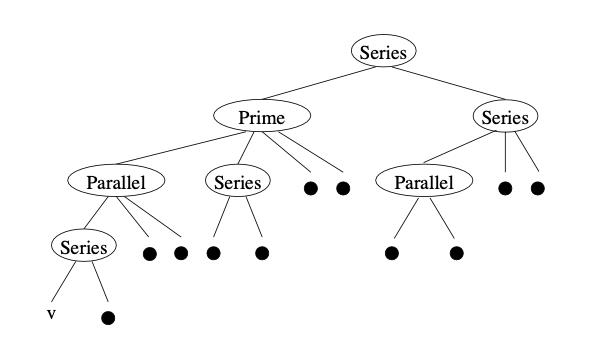
\includegraphics[width=0.80\textwidth]{images/graphs/modular-decomposition-tree}
    \caption{A modular decomposition tree}
    \label{fig:example-modular-decomposition-tree}
\end{figure}

\begin{algorithm}[H]
    \caption{Ehrenfeucht et al. \cite{SAMD}\cite{PTDMD}} % Reference citation in the caption
    \KwIn{An arbitrary vertex $v$ of $G = (V, E)$, $T = \text{spine}(G, v)$ and $\{T_X = MD(G[X]) \mid X \in \mathcal{M}(G,v)\}$}
    \KwOut{The modular decomposition tree $MD(G)$}
    \SetKwBlock{Begin}{begin}{end}
    \Begin{
        \ForEach{leaf $X$ of $T$}{
            Let $T_X = MD(G[X])$ and $p(X)$ be $X$'s father in $T$\;
            Replace $X$ by $T_X$ in $T$\;
            \If{the root $r(T_X)$ and $p(X)$ are both parallel or series}{
                Remove $r(T_X)$ and connect the children of $r(T_X)$ to $p(X)$\;
            }
        }
    }\label{alg:algorithm-Ehrenfeucht-et-al}
\end{algorithm}


\section{Advantages of Ehrenfeucht's Algorithm}\label{sec:advantages-of-ehrenfeucht's-algorithm}

\begin{itemize}
    \item \textbf{Efficiency:} The algorithm operates in $O(n^2)$ time, making it feasible for large graphs.
    \item \textbf{Simplicity:} The divide-and-conquer approach simplifies the process of identifying modules and constructing the decomposition tree.
    \item \textbf{Practicality:} The algorithm is applicable to both undirected graphs and 2-structures.
\end{itemize}


\hspace{4cm}

The next chapter will discuss an implementation of the algorithm in Python made by another Sorbonne University student and its performance compared with another implementation made in SageMath.

    %! Author = adrienkoumgangtegantchouang
%! Date = 01/10/24

\chapter{Algorithm of modular decomposition}\label{ch:algorithm-of-modular-decomposition}

Modular decomposition is a powerful technique used to simplify and analyze the structure of graphs by breaking them down into modules.
One of the notable algorithms for achieving this is the algorithm developed by Ehrenfeucht et al.
This section delves into the details of the algorithm, its steps, and its application in graph theory.

\section{Introduction of Partition Tree Family}\label{sec:introduction-of-partition-tree-family}

In the article ``An $O(n^2)$ Divide-and-Conquer Algorithm for the Prime Tree Decomposition of Two-Structure and Modular Decomposition of Graphs article\cite{PTDMD}", Ehrenfeucht and co work directly on two-structured graphs, and the application of their algorithms can easily be extended to other graph.
A two-structure is the generalization that allows an arbitrary coloring of this set.
A two-structure may thus be viewed as an edge-colored complete directed graph.
Graphs are a special case of two-structures, so all theorems and algorithms presented in this chapter for two-structures are immediately applicable to graphs.


If $g$ is a two-structure, $dom(g)$ denotes its nodes.
The substructure induced in $g$ by $X \subseteq dom(g)$, denoted $g \mid X$, is the subgraph of $g$ induced by $X$, where the edges in $g \mid X$ have the same color as they do in $g$.
A node $x$ distinguishes nodes $y$ and $z$ if $(x, y)$ and $(x, z)$ are different colors,or $(y, x)$ and $(z, x)$ are different colors.
A module is a set $X \subseteq dom(g)$ such that no $x \in dom(g) - X$ distinguishes any two members of $X$.
It is easily seen that if two modules are disjoint, all edges from one of the modules to the other are the same color.
If $R$ is a partition of the nodes of $g$, a system of representatives from $R$ is a set consisting of one node from each member of $R$.
If each member of $R$ is a module of $g$, then every system of representatives induces the same substructure.
This substructure is denoted $g / R$, and completely specifies the colors of all edges that are not internal to a member of $R$.
The operation may be performed recursively on each member of $R$ by partitioning it into still smaller modules.
The result is a compact, hierarchical decomposition of the entire two-structure.

The \textit{prime tree family} of a two-structure is such a hierarchical decomposition, and it is unique.
It is given by the family of \textit{prime modules} : $\{X : X$ is a nonempty module of $g$, and for any module $Y$, either $Y \subseteq X, X \subseteq Y$, or $X \cap Y = \emptyset\}$.
If $\mid X \mid > 1$, the maximal-cardinality members of the prime tree family that are proper subsets of $\mid X \mid$, denoted $children_g(X)$, are a partition of $X$.
Thus $(g \mid X) / children_g(X)$, given for all $X$ in the prime tree family, completely represents the original two-structure.
As is described below, this family represents in a simple way all modules in the two-structure, not just those that are members of the family.
The number of modules may be exponential in $n$, but this representation takes space that is linear in $n$.

The prime tree family for the case of graphs is also known as the modular decomposition\cite{IMD}.


\section{Preliminaries}\label{sec:preliminaries}

Let $G$ be a directed graph.
The \textit{component graph} for $G$ has one node for each strongly connected component.
If $X$ and $Y$ are two strongly connected components of $G$, then $(X,\, Y)$ is an edge in the component graph if there exist $x \in X$ and $y \in Y$ such that $(x,\, y)$ is an edge of $G$.

Let $X$ and $Y$ be finite sets.
$X$ and $Y$ are overlapping if and only if $X - Y$, $ X \cap Y$, and $Y - X$ are all nonempty.
A two-edge over $X$ is an ordered pair $(x,\, y)$ such that $x \neq y$ and $x, y \in X$.
In this section, the term edge refers to a two-edge.
The set $E_2(X)$ is the set of all possible edges over $X$, and a two-structure on domain $X$ is a coloring of $E_2(X)$.
An edge $(x,\, y)$ is symmetric if $(y,\, x)$ is the same color.
A two-structure is symmetric if all of its edges are symmetric.
$X$ is a singleton set if $\mid X \mid = 1$.
The nodes of a two-structure $g$ are known as its \textit{domain}, denoted $dom(g)$, and $g$ is a coloring of $E_2(dom(g))$.
Obviously, $dom(g)$, $\emptyset$, and the singleton subsets of $dom(g)$ are modules of $g$; these are the trivial modules of $g$.
In this section, modules will be assumed to be nonempty, except when otherwise stated.

Let $g$ be a two-structure, and let $R$ be a partition of $dom(g)$ such that every member of $R$ is a module of $g$.
Let $g'$ be the two-structure $g / R$.
If $X \subseteq dom(g')$, its inverse image in $g$ is the union of the members of $R$ that correspond to members of $X$.
$X$ is the image in $g'$ of its inverse image.

\begin{mytheo}
    \label{thm:2-1}
    Let $g$ be a two-structure, and let $X$ and $Y$ be overlapping modules of $g$.
    Then $\X \cap Y$, $X \cup Y$, and $X - Y$ are modules of $g$.
\end{mytheo}

\begin{mytheo}
    \label{thm:2-2}
    Let $g$ be a two-structure, and let $R$ be a partition of $dom(g)$ into modules.
    \begin{enumerate}
        \item If $X$ is a module in $g$ that has an image $Y$ in $g / R$, then Y is a module in $g / R$.
        Moreover, if $X$ is a prime module in $g$, then $Y$ is a prime module in $g / R$.
        \item If $Y$ is a module in $g / R$, then its inverse image, $X$, is a module in $g$.
        Moreover, if the members of $R$ are prime modules in $g$ and $Y$ is a prime module in $g / R$, $X$ is a prime module in $g$.
    \end{enumerate}
\end{mytheo}

\begin{mylem}
    \label{lem:2-3}
    Let $g$ be a two-structure, and let $X$ be a module of $g$.
    Then the modules of $g \mid X$ are those modules of $g$ that are subsets of $X$.
    Moreover, the prime modules of $g \mid X$ that are proper subsets of $X$ are the prime modules of $g$ that are proper subsets of $X$.
\end{mylem}


\begin{mydef}
    \label{def:2-4}
    Let $g$ be a two-structure.
    \begin{enumerate}
        \item $g$ is \textit{primitive} if and only if it contains at least three nodes and all modules in $g$ are trivial.
        \item $g$ is \textit{complete} if and only if all of its edges are the same color.
        \item $g$ is \textit{linear} if and only if there exists a linear order $(x_1, \dots, x_{\mid dom(g) \mid})$ of the elements of $dom(g)$ such that the edges $\{(x_i,\, x_j): i < j\}$ are the same color, the edges $\{(x_j,\, x_i): i < j\}$ are the same color, and the colors of these two sets are different.
    \end{enumerate}
\end{mydef}

It is clear that if $g$ is complete, its modules are all subsets of $dom(g)$, and if it is linear, then its modules are the consecutive sets (sets of the form $\{x_i, x_{i+1}, \dots, x_j\}$) in the linear order on its nodes.

\begin{mytheo}[primitive, complete and linear]
    \label{thm:2-5}
    .\\
    \begin{enumerate}
        \item If $X$ is a prime module of $g$ and $\mid X \mid > 1$, $children_g(X)$ is a partition of $X$;
        \item Each module of a two-structure $g$ is a union of siblings in the prime tree family of $g$;
        \item If $X$ is a prime module of $g$ such that $\mid X \mid > 1$, $X$ is of one of the following types:
            \begin{itemize}
                \item \textbf{primitive}: no union of more that one and less than all of its children is a module of $g$;
                \item \textbf{complete}: every union of a subfamily of its children is a module of $g$;
                \item \textbf{linear}: there exists a linear ordering on its children such that the union of a subfamily is a module of $g$ if and if the subfamily is consecutive in that ordering.
            \end{itemize}
    \end{enumerate}
\end{mytheo}

\begin{mycor}
    \label{cor:2}
    If $X$ is a member of the prime tree family, then $(g \mid X) / children_g(X)$ is either \textit{primitive}, \textit{linear}, or \textit{complete}.
\end{mycor}

By Theorem~\ref{thm:2-5}, we way represent all modules of $g$ as follows.
Create one node to represent each prime module.
If $x$ represents a prime module $X$, establish an edge from $x$ to $y$ whenever $y$ represents a member of $children_g(X)$.
We will call this data structure $ptf(g)$.
In $ptf(g)$, the leaf descendants of node $x$ give the prime module $X$ it represents.
In addition, if $\mid X \mid > 1$, one may label $x$ as primitive, linear or complete, and supply the appropriate ordering of its children if it is linear.
If $x$ is complete, its color is the color of the edges connecting its children.
If $x$ is linear, its colors are the two colors of edges connecting its chidlren.

We seek to compute $ptf(g)$.
For ease of notation, when $x$ is a node of $ptf(g)$ that represents a prime module $X$, we will view $x$ and $X$ as synonymous.


\section{The Algorithm}\label{sec:the-algorithm}

In this section, we give an algorithm that computes $ptf(g)$ for symmetric two-structures.
Since undirected graphs are symmetric two-structures, they are covered.
Later, we will give the minor modification needed when the two-structure may have asymmetric edges.
We will assume that the two-structure is given as an adjacency array, and that if the two-structure has $k$ edge colors, they are given in the adjacency array as integers from zero to $k-1$.

$G(g, v)$ is trivially computed in $O(n^2)$ time. $M(g, v)$ is a partition of $dom(g) - \{v\}$, and it may be computed with Algorithm~\ref{alg:compute}, variants of which have appeared repeatedly in related contexts.
The prime tree family of an arbitrary two-structure is then computed with Algorithm~\ref{alg:ptf}.


\begin{mydef}
    \label{def:3-1}
    Let $u$ be a node of $dom(g)$; $G(g, u)$ denotes a graph whose nodes are given by $dom(g) - (0)$.
    There is an edge in $G(g, v)$ from node $x$ to node $y$ if $x$ distinguishes $y$ and $v$ in $g$.
    $M(g,u)$ denotes the family of maximal modules of $g$ that do not contain $v$.
    That is, $X \in M(g, 0)$ iff $X$ is a module, and for every module $Y$ such that $X \subset Y$, $Y$ contains $v$.
\end{mydef}


\begin{algorithm}[H]
    \label{alg:compute}
    \SetAlgoLined
    \caption{Compute M(g, v)}
    Maintain a family $L$ of partition classes, and for each partition class $S$, maintain a set $Z(S)$ of "unprocessed outsiders".\\
    Initially, there is one partition class $S = \text{dom}(g) - \{u\}$ in $L$, with $Z(S) = \{u\}$.

    \While{$L$ contains a class $S$ such that $Z(S)$ is nonempty}{
        Remove $S$ from $L$\;
        Let $w$ be an arbitrary member of $Z(S)$\;
        Partition $S$ into the maximal subsets that are not distinguished by $w$\;
        \For{each resulting subset $W$}{
            Make $W$ a member of $L$\;
            Let $Z(W) = (S - W) \cup (Z(S) - \{w\})$\;
        }
    }
\end{algorithm}


\begin{algorithm}[H]
    \caption{ptf(g)}
    \label{alg:ptf}
    Select a node $u$ of $g$ and compute $M(g, u)$ using Algorithm \ref{alg:compute}\;
    Let $g' = g / (M(g, u) \cup \{\{u\}\})$\;
    Let $u'$ be the image of $u$ in $g'$\;
    Let $G' = G(g', u')$\;
    Let $G''$ be the component graph of $G'$\;
    Create a tree node $t$\;
    $u := t$\;
    \While{$G''$ is not empty}{
        Create a tree node $w$ and make it a child of $u$\;
        Remove a sink from $G''$; let $F$ be the corresponding members of $M(g, u)$\;
        \eIf{$\mid F \mid > 1$}{
            $u$ is primitive\;
        }{
            $u$ is complete\;
        }
        \ForEach{member $X$ of $F$}{
            Compute $ptf(g \mid X)$ recursively\;
            \eIf{$u$ and the root of $ptf(g \mid X)$ are both complete and have the same color}{
                Make the children of $ptf(g \mid X)$ be children of $u$\;
            }{
                Make $ptf(g \mid X)$ be a child of $u$\;
            }
        }
        $u := w$\;
    }
    \Return $t$\;
\end{algorithm}


\section{Correctness and Time bound}\label{sec:correctness-and-time-bound}

\subsection{Algorithm \ref{alg:compute}}\label{subsec:algorithm-compute}

\begin{mylem}
    \label{lem:lemma-4-1}
    Let $g$ be a two-structure, and let $v \in dom(g)$.
    Then $M(g, v) \cup \{\{v\}\}$ is a partition of $dom(g)$.
\end{mylem}

\textbf{Proof.}
If a node $w \neq v$ is not in any member of $M(g, v)$, then there is no module containing $w$ but excluding $v$, contradicting the fact that $\{w\}$ is such a module.
Suppose $w$ is in two members, $X$ and $Y$, of $M(g, v)$.
The union of $X$ and $Y$ is a module that does not contain $v$, since one contains the other or else they overlap, in which case their union is a module by Theorem~\ref{thm:2-1}.
They cannot both be maximal modules not containing $v$, contradicting membership of both of them in $M(g, v)$.
Thus, each node of $dom(g) - \{v\}$ is a member of exactly one set in $M(g, v)$.
$M(g, v)$ is a partition of $dom(g) - \{v\}$, and the lemma follows.


\begin{mylem}
    \label{lem:4-2}
    Algorithm~\ref{alg:compute} computes $M(g, v)$.
\end{mylem}

\textbf{Proof.}
The algorithm clearly maintains the following invariant: For each partition class $S$, a member $x$ of $dom(g) - S$ may distinguish members of $S$ only if it is a member of the outside list for $S$.
The algorithm terminates when every outsider list is empty, hence, when each partition class in a module.
Conversely, if a module of $g$ does not contain $v$, it is a subset of the initial member of $L$, and its members cannot be split into different partition classes by any outsider.
Thus, its memebers are all in the same final partition class.
Since each maximal module that does not contain $v$ is a final partition class, the final partition classes must be the maximal modules that do not contain $v$, by Lemma~\ref{lem:lemma-4-1}.

\begin{mydef}
    \label{def:4-3}
    Let $g$ be a two-structure, and let $R$ be a partition of $dom(g)$.
    The edges that are exposed by $R$ are the set $\{(u, v): u, v \in dom(g)$ and $u$ and $v$ are not in the same partition class of $R\}$
\end{mydef}

\begin{mylem}
    \label{lem:4-4}
    Let $g$ be a two-structure, let $v \in dom(g)$, and let $k$ be the number of edges exposed by $M(g, v) \cup \{\{v\}\}$.
    The number of operations required by Algorithm~\ref{alg:compute} is $O(k)$.
\end{mylem}

\textbf{Proof.}
Maintain all sets $L$ and their outsider sets as linked lists.
A set $S$ may be partitioned with an outsider $w$ in $O(\mid S \mid)$ time as follows.
Use a two-phase bucket sort.
In the first phase, bucket sort the members of $S$ according to the color of the edges from $w$ to those members.
In the second phase, bucket sort each of the resulting nonempty buckets according to the colors of the edges from those members to $w$.
Charge the cost of the partition to the edges connecting w and the members of $S$.
Charge the cost of having originally inserted $w$ on the outsider set for $S$ to one of these edges.
Since w is not on any of the new outsider sets, these edges do not receive any further charges in later iterations, so they are each charged constant cost over all executions.
Only exposed edges receive charges.
Thus, the costs of performing all partitions and maintaining all lists is $O(k)$.

\subsection{Algorithm \ref{alg:ptf}}\label{subsec:algorithm-ptf(g)}

\begin{mylem}
    \label{lem:5-1}
    Let $g$ be a two-structure, and let $v \in dom(g)$, where $\mid dom(g) \mid > 1$.
    Let $U \neq \{v\}$ be a proper ancestor of $\{v\}$ in $ptf(g)$, and let $W$ be $U$'s child that contains $v$:
    \begin{enumerate}
        \item If $(g \mid U) / children_g(U)$ is primitive, each of $U$'s children, other than $W$, is a member of $M(g, v)$.
        \item If $(g \mid U) / children_g(U)$ is complete, the union of all of $U$'s children except $W$ is a member of $M(g, v)$.
        \item If $(g \mid U) / children_g(U)$ is linear, the union of children of $U$ that are before $W$ in the linear order is a member of $M(g, v)$ or empty.
        The same is true of any children after $W$.
    \end{enumerate}

    There are no members of $M(g, v)$ other than those given by the above rule when it is applied to all ancestors of $v$.
\end{mylem}

\textbf{Proof.}
Follows from Theorem~\ref{thm:2-5}

\begin{mytheo}
    \label{thm:5-2}
    Let $g' = g / (M(g, v) \cup \{\{v\}\})$.
    If $g$ is symmetric, then the modules of $g'$ that contain the image of $\{v\}$ are prime in $g'$, and their inverse images in $g$ give the ancestors of $\{v\}$ in the prime tree family of $g$.
\end{mytheo}

\textbf{Proof.}
Suppose $U$ is a proper ancestor of $(v)$ in the prime tree family of $g$ and $W$ is its child that contains $v$.
By Lemma~\ref{lem:5-1} , $U$ and $W$ are the inverse images of sets of nodes of $g'$.
By Theorem~\ref{thm:2-2}, their images in $g'$ are prime in $g'$.
If $g$ is symmetric, $U$ is complete or primitive, so by Theorem~\ref{thm:2-2} and Lemma~\ref{lem:5-1}, the image of $U$ is the smallest module of $g'$ that contains the image of $W$.
Applying this argument to all ancestors $U$ of $(v)$ shows that all modules of $g'$ that contain the image of $(u)$ are the images
of the ancestors of $(v)$ in the prime tree family of $g$.

\begin{mylem}
    \label{lem:5-3}
    Let $g$ be a two-structure, and let $X$ be the set of nodes reachable from node $x$ in $G(g, v)$.
    The set $dom(g) - X$ is the largest module of $g$ that contains $u$ and excludes $x$.
\end{mylem}

\textbf{Proof.}
If there is an edge from $x$ to $y$ in $G(g, v)$ then $(x, y)$ and $(x, v)$ are different colors or $(y, x)$ and $(v, x)$ are different colors, which means that any module containing u and excluding x must also exclude y.
If $y$ is excluded from the module, then the same argument shows that any node reachable from $y$ on a single edge must also be excluded from the module.
Transitively, every node reachable from $x$ on any path must be excluded from the module.
To see that $dom(g) - X$ is, in fact, a module, we observe that the nodes in $dom(g) - X$ are not reachable in $G(g, u)$ from any node in $X$, which means that for any node $z$ in $X$ and any node $u$ in $dom(g) - $X, $(z, u)$ and $(z, v)$ are the same color and $(u, z)$ and $(v,z)$ are the same color.
Transitively, for any two nodes u and w in $dom(g) - X$, $(z, u)$ and $(z, w)$ are the same color and $(u, z)$ and $(w, z)$ are the same color.
Thus, $dom(g) - X$ is a module.

\begin{mycor}
    \label{cor:}
    Let $X$ be a set corresponding to a sink in the component graph of $G(g, v)$.
    Then $dom(g) - X$ is a maximal-cardinality module that contains $v$ and that is not equal to $dom(g)$.
\end{mycor}

\begin{mypro}
    \label{prop:5-4}
    Let $g$ be a two-structure, let $v \in dom(g)$, and let $X \subseteq dom(g) - \{v\}$.
    Let $g' = g \mid (dom(g) - X)$.
    Then $G(g', v)$ is the sub-graph induced in $G(g, v)$ by $dom(g) - (X \cup \{v\})$.
\end{mypro}

\begin{mytheo}
    \label{thm:5-5}
    Let $g$ be a two-structure, and let $W$ be a child of $U$ in $ptf(g)$.
    If $U$ and $W$ are both complete, the color of the edges connecting children of $W$ is different from the color of the edges connecting children of $U$.
    If $U$ and $W$ are both linear, the pair of colors of edges connecting children of $W$ is different from the pair of colors connecting children of $U$.
\end{mytheo}

The correctness of Algorithm~\ref{alg:ptf} now follows.
Algorithm~\ref{alg:ptf} clearly returns the correct result whenever $\mid dom(g) \mid = 1$.
Let the inductive hypothesis be that it returns the correct result whenever $\mid dom(g) \mid < k$.
Suppose that $\mid dom(g) \mid = k$.
Let $W$ be the child of $dom(g)$ in $ptf(g)$ that contains $v$, and let $g' = g/(M(g,u) \cup \{\{v\}\}$.
By Theorem~\ref{thm:5-2}, there is a unique maximal module of $g'$ that is a proper subset of $dom(g')$ and that contains the image of $\{v\}$.
Thus, by the corollary to Lemma~\ref{lem:5-3}, there is a unique sink in the component graph for $G(g',u')$.
By Theorem~\ref{thm:5-2}, $W = dom(g') - \cup F$.
The characterization of $U$ as primitive or complete is correct, by Lemma~\ref{lem:5-1}.
By the inductive hypothesis, the recursive call produces the correct tree for $g \mid X$, so by Lemma~\ref{lem:2-3} and Theorem~\ref{thm:5-5}, the main routine correctly attaches all siblings of $W$ and their descendants as children of $dom(g)$.
By Proposition~\ref{prop:5-4} and Lemma~\ref{lem:2-3}, subsequent iterations of the main loop of Algorithm~\ref{alg:compute} are computationally equivalent to a recursive call to Algorithm~\ref{alg:compute} on $g \mid W$.
By the inductive hypothesis, they produce the subtree of $ptf(g)$ rooted at $W$.
Thus, Algorithm~\ref{alg:compute} produces the correct result when $\mid dom(g) \mid \leq k$.
Inductively, it produces the correct result for all symmetric two-structures.

For the time bound, let $k$ be the number of edges exposed by $M(g, v) \cup \{\{v\}\}$.
If the two-structure has only one node, we may charge the cost of returning the trivial decomposition to the node.
Otherwise, by Lemma~\ref{lem:4-4}, computing$ M(g, v)$ requires $O(k)$ time, so we may charge this cost to the exposed edges.
Let $g' = g/(M(g, v) \cup \{\{v\}\})$.
The number of nodes of g' is $O(k^{1/2})$.
Computing $G(g',v')$ and the component graph of $G(g', v')$ takes $O(k)$ time, as does the cost of identifying and removing sinks from the component graph.
These costs may be charged to the exposed edges at constant cost per edge.
In recursive calls, we use the same charging scheme on edges exposed in those calls.
Each recursive call generated from the main procedure occurs on the substructure induced by a single member of $M(g, v)$, and thus, the edges charged in one recursive call are disjoint from those charged in either the main procedure or any other recursive call.
It follows that all costs are charged to the edges at constant time per edge, giving the $O(n^2)$ time bound on the algorithm.



\section{The generalization of Algorithm \ref{alg:ptf} for arbitrary Two-Structure}\label{sec:the-generalization-of-algorithmref{alg:ptf}-for-arbitrary-two-structure}

Algorithm~\ref{alg:3} gives the generalization of Algorithm~\ref{alg:ptf} for arbitrary two-structures.
For the correctness, note that when asymmetric edges are allowed, case 3 of Lemma\ref{lem:5-1} can no longer be excluded.
Because of this, Theorem~\ref{thm:5-2} is no longer true.
Instead, we make use of the following.

\begin{mylem}
    \label{lem:6-1}
    Let $g$ be a two-structure, let $v$ be a node of $g$, and let $W$ be the child of $dom(g)$ that contains $v$.
    Let $g' = g / (M(g, v) \cup \{\{v\}\})$, let $v'$ be the image of $v$ in $g'$, and let $W'$ be the image of $W$.
    Let $G''$ be the component graph of $G(g', v')$, and let $X'$ be the nodes of $g'$ that correspond to the sinks of $G''$.
    Then $W' = dom(g') - X'$.
\end{mylem}

\textbf{Proof.}
By Lemma~\ref{lem:5-1}, $W$ has an image in $g'$, and by Theorem~\ref{thm:2-2}, $W'$ is prime in $g'$.
By Theorem~\ref{thm:2-2}, if the root of $ptf(g)$ is primitive, $W'$ is the unique maximal module of $g'$ that contains $v'$ and that is not equal to $dom(g')$.
If the root of $ptf(g)$ is complete, then by Theorem~\ref{thm:2-2} and Lemma~\ref{lem:5-1}, $W'$ has only one sibling in $ptf(g')$, so it is again the unique maximal module of $g'$ that contains $v'$ and that is not equal to $dom(g')$.
In either case, Lemma~\ref{lem:6-1} is true by the corollary to Lemma~\ref{lem:5-3}.
If the root of $ptf(g)$ is linear, then by Theorem~\ref{thm:2-2} and Lemma~\ref{lem:5-1}, $ W'$ has one or two siblings in $ptf(g')$.
If it has one sibling, it is the unique maximal module of $g'$ that contains $v'$ and that is not equal to $dom(g')$, so again, the lemma is true.
Otherwise, the union of $W'$ and either of these siblings is thus a maximal module of $g'$ that contains v and is not equal to $dom(g)$.
Thus, each of these siblings is a sink of $G''$, by the corollary to Lemma~\ref{lem:5-3}.
These are the only sinks of $G''$, since $W'$ is prime in $g'$.
Thus, the lemma is true in this case also.


The proof of correctness of Algorithm~\ref{alg:3} is similar to the one for Algorithm~\ref{alg:ptf}: Algorithm~\ref{alg:3} clearly returns the correct result whenever $\mid dom(g) \mid = 1$.
Let the inductive hypothesis be that it returns the correct result whenever $\mid dom(g) \mid < k$.
Suppose $\mid dom(g) \mid = k$.
Let $W$ be the child of $dom(g)$ in $ptf(g)$ that contains 4, and let $g' = g/(M(g, u) \cup \{\{v\}\})$.
Let $X'$ be the nodes of g' that correspond to the sinks of $G''$.
By Lemma~\ref{lem:6-1}, $W$ is the inverse image of $dom(g') - X'$.
The characterization of u as primitive is correct, by Lemma~\ref{lem:5-1}.
If there are two sinks in $G''$, $u$ is linear.

Otherwise, it is linear or complete.
Which case holds may be found by examining whether an edge such as $(v, x)$ that connects its children is symmetric.
By the inductive hypothesis, the recursive call produces the correct tree for $g \mid X$, for each $X$ e $M(g,v)$, so by Lemma~\ref{lem:2-3} and Theorem~\ref{thm:5-5}, the main routine correctly attaches all siblings of $W$ and their descendants as children of $dom(g)$.
By Proposition~\ref{prop:5-4} and Lemma~\ref{lem:2-3}, subsequent iterations of the main loop of Algorithm~\ref{alg:3} are computationally equivalent to a recursive call to Algorithm~\ref{alg:3} on $g \ mid W$.
By the inductive hypothesis, they produce the subtree of $ptf(g)$ rooted at $W$.
Thus, Algorithm~\ref{alg:3} produces the correct result when $\mid dom(g) \mid \leq k$.
Inductively, it produces the correct result for all two-structures.

The proof of the $O(n^2)$ time bound for Algorithm~\ref{alg:3} is identical to the one for Algorithm~\ref{alg:ptf}.

\begin{algorithm}[H]
    \caption{ptf(g)}
    \label{alg:3}
    Select an arbitrary node $v$ of $g$ and compute $M(g, v)$\;
    Let $g' = g / (M(g, v) \cup \{\{v\}\})$\;
    Let $(v')$ be the image of $\{v\}$ in $g'$\;
    Let $G' = G(g', u')$\;
    Let $G''$ be the component graph of $G'$\;
    Create a tree node $t$\;
    Let $u := t$\;
    \While{$G''$ is not empty}{
        Create a tree node $w$ and make it a child of $u$\;
        Remove all sinks from $G''$; let $F$ be the corresponding members of $M(g, v)$\;
        \eIf{only one sink was removed from $G''$ and $\mid F \mid > 1$}{
            $u$ is primitive\;
        }{
            Select an arbitrary node $x$ from a member of $F$\;
            \eIf{$(v, x)$ and $(x, v)$ are the same color}{
                $u$ is complete\;
            }{
                $u$ is linear\;
            }
        }
        \ForEach{member $X$ of $F$}{
            Compute $ptf(g|X)$ recursively\;
            \eIf{$u$ and the root of $ptf(g \mid X)$ are both complete and the same color or both linear and the same color}{
                Make the children of $ptf(g \mid X)$ be children of $u$\;
            }{
                Make $ptf(g \mid X)$ be a child of $u$\;
            }
        }
        $u := w$\;
    }
    \Return $t$\;
\end{algorithm}


\section{Advantages of Ehrenfeucht's Algorithm}\label{sec:advantages-of-ehrenfeucht's-algorithm}

\begin{itemize}
    \item \textbf{Efficiency:} The algorithm operates in $O(n^2)$ time, making it feasible for large graphs.
    \item \textbf{Simplicity:} The divide-and-conquer approach simplifies the process of identifying modules and constructing the decomposition tree.
    \item \textbf{Practicality:} The algorithm is applicable to both directed, undirected, and 2-structures graphs.
\end{itemize}


\hspace{4cm}

The next chapter will discuss an implementation of the algorithm in Python made by another Sorbonne University student and its performance compared with another implementation made in SageMath.



% Implementation in SageMath and Python
    %! Author = adrien koumgang tegantchouang
%! Date = 09/07/24

\chapter{Previous Work: Implementation in SageMath and Python by Pistiloglou’s}\label{ch:previous-work-implementation-in-sagemath-and-python}

\section{Implementation in SageMath}\label{sec:implementation-in-sagemath}

SageMath~\cite{sagemathtour} is built out of hundreds of open-source packages and features a unified interface.
SageMath can be used to study elementary and advanced, pure and applied mathematics.
This includes a huge range of mathematics, including basic algebra, calculus, elementary to very advanced number theory, cryptography, numerical computation, commutative algebra, group theory, combinatorics, graph theory, exact linear algebra and much more.
It combines various software packages and seamlessly integrates their functionality into a common experience.
It is well-suited for education and research.


\section{Overview of Eleni Pistiloglou's Project and implementation in Python}\label{sec:overview-of-eleni-pistiloglou's-project-and-implementation-in-python}

Eleni Pistiloglou, in her ``Rapport de projet''\cite{DM2S} for the Master 1 Informatique, parcours STL, in 2021, has made significant contributions to modular decomposition implementation by implementing modular decomposition algorithms in Python.
Its implementation follows that of SageMath and its role is to improve the performance of the SageMath implementation.
This section provides an overview of her work, highlighting the methodologies and results of her implementations, which later served as a foundation for my work in converting the Pistiloglou’s Python implementation to Rust.

Eleni Pistiloglou's project focuses on the modular decomposition of 2-structures, specifically directed graphs with colored arcs.
Her work involves:
\begin{itemize}
    \item Defining key concepts such as modules and maximal modular partitions.
    \item Implementing modular decomposition algorithms.
    \item Evaluating and comparing the performance of these implementations in Python.
\end{itemize}

Python, a high-level programming language known for its simplicity and versatility, was also used by Pistiloglou to implement the modular decomposition algorithm.
The following are the results.

Firstly, the initial version of the code defines a TwoStructure class to represent a 2-structure that uses a dictionary to store arcs, whose key is the source index and whose value is a dictionary containing the destinations associated with the colour.
So the call to the function that decides whether a node distinguishes two others requires access to the values of both dictionaries.
Similarly, for the function that returns the colour of an arc.
The theoretical complexity of a dictionary search is $O(1)$ thanks to hashing, but implementing dictionary operations in Python is very time-consuming.
So her first attempt was to determine the most suitable data structures for representing the arcs and colours of a 2-structure and to design a new implementation for the parts that were dictionary-based.

The second version proposes an improved implementation of these functions that is possible using only sets or lists.
Sets are preferred over lists because their elements can be retrieved in $O(1)$ time thanks to hashing, unlike a search in a list, which is performed in $O(n)$ time.
Since the number of colours in a 2-structure is much smaller than the number of its arcs, a storage system that associates colours with source-destination pairs would improve the speed of calculation, which would be carried out in $O(K) \cdot O(1)$ time with k the number of arc colors in the graph.
A bucket-sort solution stores each arc in an arc set that contains only arcs of the same colour.
The sets are stored in a list whose index corresponds to the colour of the arcs contained in that set.
The code for these two versions is available in her report.
She made other significant improvements to almost 50\% of the initial functions to adapt them to the changing data structures and to improve their completeness.
As a result, when tested on randomly structured graphs with 1000 nodes and 100 arcs, the total execution time for decomposing a directed graph was reduced to 0.152s in the second version, compared with 5.448s before the improvements.
Performance was also compared with SageMath on undirected graphs.
However, SageMath performed significantly better, with a latency twice as high as SageMath on graphs with 100 arcs.
For much larger graphs, such as 1000 arcs, we obtain an execution time of around 5 minutes with Pistiloglou implementation and 0.7 seconds with SageMath.
All these results can be found in her report.




% Implementation in Rust and C++
    %! Author = adrien koumgang tegantchouang
%! Date = 09/07/24


\chapter{Implementation in Rust and C++}\label{ch:implementation-in-rust-and-cpp}

The implementation of the modular decomposition algorithm in Rust was motivated by the need to overcome performance limitations observed in previous implementation in Python.
The primary motivation for implementing the modular decomposition algorithm in Rust was to achieve better performance and scalability for large and complex graphs.
As described on the official Rust website, we have that Rust is blazingly fast and memory-efficient: with no runtime or garbage collector, it can power performance-critical services, run on embedded devices, and easily integrate with other languages.
Rust's rich type system and ownership model guarantee memory-safety and thread-safety -- enabling you to eliminate many classes of bugs at compile-time.
In brief, Rust is a programming language that adopts a very specific programming philosophy, mainly thanks to its ownership principle, which ensures memory safety without needing a garbage collector.
Ownership governs how memory is managed and how different parts of a program can access and modify data.

The key principles of ownership in Rust are~\cite{rust}:
\begin{itemize}
    \item \textbf{Ownership Rules}
    \begin{itemize}
        \item Each value in Rust has a variable that's called its owner.
        \item There can only be one owner at a time.
        \item When the owner goes out of scope, the value will be dropped (freed).
    \end{itemize}
    \item \textbf{Borrowing and References}
    \begin{itemize}
        \item A variable can borrow a value by creating a reference to it using `\&'.
        \item Borrowing can be either immutable (`\&T') or mutable (`\&mut T').
        \item Multiple immutable references are allowed, but only one mutable reference is allowed at a time.
    \end{itemize}
    \item \textbf{Move Semantics}
    \begin{itemize}
        \item When a value is assigned to another variable or passed to a function, the ownership of the value moves to the new variable or function parameter.
        \item After the move, the original variable is no longer accessible.
    \end{itemize}
    \item \textbf{Copy Trait}
    \begin{itemize}
        \item For types that implement the `Copy' trait (like integers and other simple types), a copy of the value is made rather than moving ownership.
    \end{itemize}
    \item \textbf{Lifetimes}
    \begin{itemize}
        \item Every ownership and every borrowing has a ``lifetime", which is the portion of the program along which it is active.
        \item Lifetimes are used by the Borrow Checker to check statically that the above rules are respected.
        \item Lifetimes ensure that references are valid as long as they are needed.
        \item They help the compiler reason about how long references should be valid and prevent dangling references.
    \end{itemize}
\end{itemize}

Coming as I do from programming languages such as C and Java, where you could have several pointers to a memory space in modification mode, where you could pass a pointer to a variable while still retaining control over it in write mode, Rust came to me as a real challenge.
The level of challenge was even greater because the code to be translated into Rust is written in Python~\cite{pythoncode}, which has the merit of being very flexible in terms of typing, variable access and memory areas~\cite{python}.
Many of the functions to be translated, especially the main one, were recursive, and some of them contained cycles that defined variables with a fairly complex life cycle.
As a result, I quickly ran into difficulties writing the code in Rust.
To overcome this, I turned to a programming language that has strongly influenced Rust: C++~\cite{cpp}.

This chapter provides an in-depth discussion of the methodologies, challenges and results associated with the implementation in Rust and the reasons why I decided to implement the algorithm also in C++.


\section{Implementation in Rust: Graph Representation, Algorithm Design and Optimization Techniques}\label{sec:implementation-in-rust:-graph-representation-algorithm-design-and-optimization-techniques}

This section delves into the detailed aspects of implementing the algorithm in Rust, covering the graph representation, algorithm design, and optimization techniques.

\subsection{Graph Representation}\label{subsec:graph-representation}

For the representation of the various graphs used during the execution of the modular decomposition algorithm, such as the 2-structures, I followed the implementation made by Eleni Pistiloglou in her second implementation in Python, which uses mainly sets instead of lists to optimise access to both nodes and arcs.

\subsubsection{2-structure}

We therefore have the following definition for the representation of a 2-structure:
\begin{lstlisting}[language=Rust, style=rust, caption={Defining the 2-structure}, label={lst:rust-define-twostructure}, firstnumber=1]
    #[derive(Debug)]
    #[derive(Clone)]
    pub struct TwoStructure {
        /// the graph of a two structure
        pub nodes: HashSet<u64>,
        /// list of sets, colors[i] contains the set of edges of color i
        pub colors: Vec<HashSet<(u64, u64)>>,
        /// only for quotient graph, contains the nodes of the graph if they are modules
        pub modules: Vec<HashSet<u64>>,
    }
\end{lstlisting}
Where we have:
\begin{itemize}
    \item \textbf{nodes}: the nodes of a two structure
    \item \textbf{colors}: list of sets, colors[i] contains the set of edges of color i
    \item \textbf{modules}: only for quotient graph, contains the nodes of the graph if they are modules
\end{itemize}

\subsubsection{SCC}

SCC, for Strongly Connected Components, is a structure that takes a graph as input and determines the `strongly connected components' of this graph using its two visit\ref{subsubsec:visit-for-scc-structure} and compute\ref{subsubsec:compute-for-scc-structure} functions.
For doing this, we use `Tarjan's strongly connected components algorithm'~\cite{sccalgowikipedia}.
Tarjan's strongly connected components algorithm is an algorithm in graph theory for finding the strongly connected components (SCCs) of a directed graph.
It runs in linear time, matching the time bound for alternative methods including Kosaraju's algorithm and the path-based strong component algorithm.
The algorithm is named for its inventor, Robert Tarjan.

\begin{lstlisting}[language=Rust, style=rust, caption={Defining the SCC}, label={lst:rust-define-scc}, firstnumber=1]
    pub struct SCC<'a> {
        pub graph: Box<dyn GraphTrait + 'a>,
        pub index: u64,
        pub components: Vec<HashSet<u64>>,
        pub comp_index: u64,
        pub dfs_stk: Vec<SCCNode>,
        pub visited: HashMap<u64, SCCNode>,
    }
\end{lstlisting}

\begin{itemize}
    \item \textbf{graph}: This attribute holds the graph on which Tarjan's algorithm will be executed.
    It provides the vertices and the adjacency list needed to traverse the graph.
    \item \textbf{index}: This attribute is used to assign a unique discovery index to each vertex when it is first visited during the depth-first search (`DFS').
    It is incremented with each new vertex visit.
    \item \textbf{components}: This attribute stores the strongly connected components (`SCCs') identified in the graph.
    Each SCC is represented as a set of vertices, and all such sets are collected in this list.
    \item \textbf{comp\_index}:
    \item \textbf{dfs\_stk}: This attribute acts as a stack to manage the depth-first search traversal.
    It helps in tracking the current path and managing backtracking, which is essential for updating the `lowlink' values and identifying SCCs.
    \item \textbf{visited}: This attribute keeps track of all the vertices that have been visited and their associated SCCNode instances.
    It helps in quickly checking whether a vertex has already been visited and accessing its SCCNode information.
\end{itemize}

where GraphTrait is:

\begin{lstlisting}[language=Rust, style=rust, caption={Defining GraphTrait}, label={lst:rust-define-graphtrait}, firstnumber=1]
    pub trait GraphTrait {
        fn vertices(&self) -> HashSet<u64>;
        fn successors(&mut self, v: u64) -> &HashSet<u64>;
    }
\end{lstlisting}

\subsubsection{SCCNode}

\begin{lstlisting}[language=Rust, style=rust, caption={Defining the SCCNode}, label={lst:rust-define-sccnode}, firstnumber=1]
    #[derive(Clone, Copy)]
    pub struct SCCNode {
        // original vertex ... must be hashable and unique (among vertices)
        pub vertex: u64,
        pub index: u64,
        pub lowlink: u64,
        pub on_stack: bool,
    }
\end{lstlisting}

\begin{itemize}
    \item \textbf{vertex}: This attribute holds the original vertex value from the graph.
    It uniquely identifies the vertex this `SCCNode' instance represents.
    \item \textbf{index}: This attribute holds the discovery index of the vertex.
    When a vertex is first visited, it is assigned a unique index, which essentially records the order of the vertex's discovery during the depth-first search (DFS).
    \item \textbf{lowlink}: This attribute is crucial for Tarjan's algorithm.
    The `lowlink' value of a vertex is the smallest index of any vertex that is reachable from the vertex, including the vertex itself.
    It helps in identifying the root of a strongly connected component.
    \item \textbf{on\_stack}: This attribute indicates whether the vertex is currently on the stack (`dfs\_stk') used by the algorithm.
    It is used to manage the backtracking process and to ensure that we only consider vertices that are part of the current path in the DFS\@.
\end{itemize}


\subsubsection{MiniGraph}

\begin{lstlisting}[language=Rust, style=rust, caption={Defining the Minigraph}, label={lst:rust-define-minigraph}, firstnumber=1]
    #[derive(Debug)]
    pub struct MiniGraph {
        dico: HashMap<u64, HashSet<u64>>,
    }
\end{lstlisting}

\subsubsection{DGraph}

\begin{lstlisting}[language=Rust, style=rust, caption={Defining the DGraph}, label={lst:rust-define-dgraph}, firstnumber=1]
    #[derive(Debug)]
    pub(crate) struct DGraph {
        nodes: HashSet<usize>,
        edges: Vec<HashSet<usize>>,
        modules: Vec<HashSet<usize>>,
    }
\end{lstlisting}

\begin{itemize}
    \item \textbf{nodes}: A set of nodes in the graph.
    \item \textbf{edges}: A vector where each element is a set of nodes representing edges for each node.
    \item \textbf{modules}: A vector of sets, where each set contains nodes representing a module within the graph.
\end{itemize}

\subsubsection{ComponentGraph}

\begin{lstlisting}[language=Rust, style=rust, caption={Defining the Component Graph}, label={lst:rust-define-component-graph}, firstnumber=1]
    #[derive(Debug)]
    struct ComponentGraph {
        graph: DGraph,
        components: Vec<HashSet<usize>>,
        modules: Vec<HashSet<usize>>,
    }
\end{lstlisting}

\begin{itemize}
    \item \textbf{graph}: The underlying directed graph.
    \item \textbf{components}: A vector of sets, where each set contains nodes representing a strongly connected component.
    \item \textbf{modules}: A vector of sets, where each set contains nodes representing a module within the graph.
\end{itemize}

\subsubsection{TreeNode}

\begin{lstlisting}[language=Rust, style=rust, caption={Defining the TreeNode}, label={lst:rust-define-treenode}, firstnumber=1]
    #[derive(Debug)]
    struct TreeNode {
        node_type: String,
        node_colors: Vec<usize>,
        children: Vec<TreeNode>,
        node_id: Option<usize>,
        prime_graph: Option<TwoStructure>,
    }
\end{lstlisting}

\begin{itemize}
    \item \textbf{node\_type}: A string indicating the type of the node.
    \item \textbf{node\_colors}: A vector of colors associated with the node.
    \item \textbf{children}: A vector of `TreeNode` instances representing the children of this node.
    \item \textbf{node\_id}: An optional node identifier.
    \item \textbf{prime\_graph}: An optional `TwoStructure` representing a prime graph associated with this node.
\end{itemize}

\subsection{Algorithms, Methods and functions}\label{subsec:algoithms-methods-and-functions}

Each of these data structures defined above implements functionality.
Here, we'll look at the ones that are most important during the modular decomposition.

\subsubsection{Compute for SCC structure}\label{subsubsec:compute-for-scc-structure}

The compute method is the entry point of the algorithm.
It iterates over all vertices of the graph and initiates the depth-first search (DFS) from any vertex that has not been visited yet.
The main goal of this method is to ensure that every node in the graph is processed and all SCCs are identified.

\begin{lstlisting}[language=Rust, style=rust, caption={Defining the TreeNode}, label={lst:rust-define-compute}, firstnumber=1]
    impl<'a> SCC<'a>
    {
        pub fn compute(&mut self) {
            for v in self.graph.vertices() {
                if self.visited.contains_key(&v) {
                    continue;
                }
                // v has not been visited
                let mut vnode = SCCNode::new(v, self.index);
                self.index += 1;
                vnode.on_stack = true;
                self.visited.insert(v, vnode);
                vnode.on_stack = false;
                self.visit(&RefCell::new(vnode));
            }
        }
    }
\end{lstlisting}

\subsubsection{Visit for SCC structure}\label{subsubsec:visit-for-scc-structure}

The visit method is where the depth-first search (DFS) happens.
It traverses the graph and updates the ``low-link” values that help determine the root of a strongly connected component.
The low-link value of a node is the smallest index reachable from that node, and it plays a critical role in identifying SCCs.

\begin{lstlisting}[language=Rust, style=rust, caption={Defining the Component Graph}, label={lst:rust-define-visit}, firstnumber=1]
    impl<'a> SCC<'a>
    {
        pub fn visit(&mut self, node: &RefCell<SCCNode>) -> SCCNode {
            let mut vnode = node.borrow_mut();
            
            vnode.on_stack = true;
            self.dfs_stk.push(*vnode);
    
            let s = self.graph.successors(vnode.vertex);
            match s {
                Some(h) => {
                    for w in h.clone() {
                        if !self.visited.contains_key(&w) {
                            // recurse
                            let mut wnode = SCCNode::new(w, self.index);
                            self.index += 1;
                            wnode.on_stack = true;
                            self.visited.insert(w, wnode);
                            wnode.on_stack = false;
                            wnode = self.visit(&RefCell::new(wnode));
                            vnode.lowlink = min(vnode.lowlink, wnode.lowlink);
                        } else {
                            let wnode = self.visited.get(&w).unwrap();
                            if wnode.on_stack {
                                vnode.lowlink = min(vnode.lowlink, wnode.index);
                            }
                        }
                    }
    
                    if vnode.lowlink == vnode.index {
                        let mut component = HashSet::new();
                        loop {
                            let mut wnode = self.dfs_stk.pop().unwrap();
                            wnode.on_stack = false;
                            self.visited.get_mut(&(wnode.vertex)).unwrap().on_stack = false;
                            component.insert(wnode.vertex);
                            // if wnode is vnode
                            if wnode.vertex == vnode.vertex {
                                break;
                            }
                        }
    
                        self.components.push(component);
                    }
                }
                _ => {}
            }
    
            *vnode
        }
    }
\end{lstlisting}

\subsubsection{Maximal modules}

The `maximal\_modules' function aims to find all maximal modules (subsets of nodes) in a graph that include a specific node `v'.

\begin{lstlisting}[language=Rust, style=rust, caption={Defining the maximal modules}, label={lst:rust-define-maximal-modules}, firstnumber=1]
    /// constructs M(g, v) according to the algorithm 3.1 of the article [1]
    ///
    /// # Arguments
    ///
    /// * 'g' - a two-structure
    /// * 'v' - a node of g
    ///
    /// # Returns
    ///
    /// a list of sets of nodes (modules)
    pub fn maximal_modules(g: &mut TwoStructure, v: u64) -> Vec<HashSet<u64>> {
        let mut init_module = g.nodes.clone();
        init_module.remove(&v);
        let mut partition = Vec::new();
        partition.push(init_module);
        let mut outsiders = Vec::new();
        let mut outsiders_h = HashSet::new();
        outsiders_h.insert(v);
        outsiders.push(outsiders_h);
        loop {
            if partition.is_empty() {
                panic!("Empty partition (please report)")
            }
            let mut module = HashSet::new();
            let mut index = 0;
            for i in 0..partition.len() {
                if outsiders.get(i).unwrap().len() as u64 > 0 {
                    // pick a module with outsiders
                    module = partition.get(i).unwrap().clone();
                    index = i;
                    break;
                }
            }
            if module.is_empty() {
                // if there is no module left having outsiders
                return partition;
            }

            // partition.remove(module)
            for i in 0..partition.len() {
                if *partition.get(i).unwrap() == module {
                    partition.remove(i);
                    break;
                }
            }

            let outsiders_i = outsiders.remove(index);
            // outsiders.remove(outsiders_i)


            // pick an arbitrary element
            let w = pickup(outsiders_i.clone());

            // list of sets of nodes
            let mut graph_alter = g.clone();
            let module_partition = module.clone();
            let r_modules = partition_module(&mut graph_alter, w, module_partition);
            for r_module in r_modules {
                let r_module_diff = r_module.clone();
                partition.push(r_module);
                // a = module - r_module
                let ha_alter = module.clone();
                let ha = ha_alter
                    .difference(&r_module_diff)
                    .collect::<HashSet<_>>();
                let mut a = HashSet::new();
                for &eha in ha {
                    a.insert(eha);
                }
                let mut b: HashSet<u64> = HashSet::new();
                if !outsiders_i.is_empty() {
                    for el in outsiders_i.iter() {
                        b.insert(*el);
                    }
                }
                b.remove(&w);
                outsiders.push(b);
            }
        }

        // this never happens
        // partition
    }
\end{lstlisting}

In arguments, we have:
\begin{itemize}
    \item `g': A reference to a `TwoStructure' representing the graph.
    \item `v': A node in the graph used as a reference for finding maximal modules.
\end{itemize}

and return a `Vec\textless HashSet\textless usize\textgreater\textgreater' where each `HashSet\textless usize\textgreater' represents a maximal module containing the node `v'.

\subsubsection{Partition module}

The `partition\_module' function aims to divide a given module (subset of nodes) into smaller submodules based on certain criteria related to the relationships between nodes in a graph.

\begin{lstlisting}[language=Rust, style=rust, caption={Defining the partition module}, label={lst:rust-define-partition module}, firstnumber=1]
    /// Partitions module in strong maximal modules
    ///
    /// # Arguments
    ///
    /// * 'g' - a two-structure
    /// * 'w' - the first node used for partitioning module
    /// * 'module' - a set of nodes of g to partition
    ///
    /// # Returns
    ///
    /// a list of sets of nodes
    pub fn partition_module(g: &mut TwoStructure, w: u64, module: HashSet<u64>) -> Vec<HashSet<u64>> {
        let colors_len = g.colors.len();

        // modules = [ [set() for c in g.colors] for c_ in g.colors ]
        let mut modules: Vec<Vec<HashSet<u64>>> = Vec::new();

        // is_empty = [ [True for c in g.colors] for c_ in g.colors ]
        let mut is_empty: Vec<Vec<bool>> = Vec::new();
        for _ in 0..colors_len {
            let mut vec_intern_modules_aux: Vec<HashSet<u64>> = Vec::new();
            let mut vec_intern_is_empty_aux: Vec<bool> = Vec::new();
            for _ in 0..colors_len {
                let set_inter_modules_aux: HashSet<u64> = HashSet::new();
                vec_intern_modules_aux.push(set_inter_modules_aux);
                vec_intern_is_empty_aux.push(false);
            }
            modules.push(vec_intern_modules_aux);
            is_empty.push(vec_intern_is_empty_aux);
        }

        for n in module {
            let c_w_n = g.color_of(w, n); // first color
            let c_n_w = g.color_of(n, w); // second color

            modules.get_mut(c_w_n as usize).unwrap().get_mut(c_n_w as usize).unwrap().insert(n);

            if *is_empty.get(c_w_n as usize)
                .unwrap()
                .get(c_n_w as usize)
                .unwrap()
            {
                is_empty.get_mut(c_w_n as usize)
                    .unwrap()
                    .push(false);
            }
        }

        let mut flattened: Vec<HashSet<u64>> = Vec::new();
        for m in modules {
            for s in m {
                if !s.is_empty() {
                    flattened.push(s);
                }
            }
        }
        flattened
    }
\end{lstlisting}

In Arguments, we have:
\begin{itemize}
    \item `g': A reference to a `TwoStructure' representing the graph.
    \item `w': A node in the graph used as a reference for partitioning.
    \item `module': A reference to a `HashSet<usize>' representing the module (subset of nodes) to be partitioned.
\end{itemize}

and return a `Vec\textless HashSet\textless usize\textgreater\textgreater' where each `HashSet\textless usize\textgreater' represents a submodule resulting from the partitioning process.


\subsubsection{Modular decomposition}

The `modular\_decomposition' function aims to decompose a graph into its modular components using a specified total order if provided.
It returns a hierarchical structure representing the modular decomposition.

\begin{lstlisting}[language=Rust, style=rust, caption={Defining the modular decomposition}, label={lst:rust-define-modular-decomposition}, firstnumber=1]
    fn modular_decomposition(g: &mut TwoStructure, total_order: Option<Vec<u64>>) -> TreeNode {
        if g.nodes.len() == 1 {
            let mut root = TreeNode::new();
            root.node_type = "LEAF".to_string();
            let iter = g.nodes.iter();
            let cloned_set: HashSet<u64> = iter.cloned().collect();
            root.node_id = Some(pickup(cloned_set));
            return root;
        }

        let mut total_order = total_order.unwrap_or_else(|| compute_total_order(g));
        total_order.retain(|&n| g.nodes.contains(&n));
        if total_order.is_empty() {
            total_order = compute_total_order(g);
        }

        let mut v = None;
        while let Some(node) = total_order.pop() {
            if g.nodes.contains(&node) {
                v = Some(node);
                break;
            }
        }
        let v = v.expect("No valid node found");

        let mods = maximal_modules(g, v);
        let mut qg = build_quotient(g, mods, v);
        let dg = build_distinction_graph(&mut qg, v);
        let mut cg = ComponentGraph::new(dg);

        let mut root = TreeNode::new();
        let mut u = &mut root;
        u.prime_graph = Some(qg.clone());

        while !cg.is_empty() {
            let mut w = TreeNode::new();
            w.node_type = "LEAF".to_string();
            w.node_id = Some(v);
            u.add_child(w);

            // get a mutable reference to the last child
            let u_ref = u;
            u = u_ref.children.last_mut().unwrap();

            let sinks = cg.remove_sinks();
            let mut fmodules: HashSet<u64> = HashSet::new();
            for sink in &sinks {
                for &mod_ in sink {
                    fmodules.insert(mod_);
                }
            }

            if sinks.len() == 1 && fmodules.len() > 1 {
                u.node_type = "PRIME".to_string();
                u.prime_graph = Some(qg.clone());
            } else {
                let iter = fmodules.iter();
                let p = pickup(iter.cloned().collect());
                let ntm = qg.node_to_module(p);
                match ntm {
                    Some(value) => {
                        let x = pickup((*value).clone());
                        if g.color_of(x, v) == g.color_of(v, x) {
                            u.node_type = "COMPLETE".to_string();
                            u.node_colors = vec![g.color_of(v, x)];
                        } else {
                            u.node_type = "LINEAR".to_string();
                            u.node_colors = vec![g.color_of(x, v), g.color_of(v, x)];
                        }
                    }
                    _ => {}
                }
            }

            for &fmod in &fmodules {
                let ntm = qg.node_to_module(fmod);
                match ntm {
                    Some(value) => {
                        let mut fg = g.slice((*value).clone());
                        let dtree = modular_decomposition(&mut fg, Some(total_order.clone()));
                        if ((u.node_type == "COMPLETE" && dtree.node_type == "COMPLETE")
                            && (u.node_colors == dtree.node_colors))
                            || ((u.node_type == "LINEAR" && dtree.node_type == "LINEAR")
                            && (u.node_colors == dtree.node_colors)) {
                            u.children.extend(dtree.children);
                        } else {
                            u.children.push(dtree);
                        }
                    }
                    _ => {}
                }
            }
        }
        root
    }
\end{lstlisting}

In arguments, we have:
\begin{itemize}
    \item `g': A mutable reference to a `TwoStructure' representing the graph to be decomposed.
    \item `total\_order': An optional vector of `u64' values specifying a total order of nodes.
    If provided, this order influences the decomposition process.
\end{itemize}

and return a `TreeNode' representing the hierarchical structure of the modular decomposition.

\hspace{4cm}


The code of all methods and functions defined in this stay in my GitHub repository~\cite{rustcode};


\section{Implementation in C++}\label{sec:implementation-in-c++}

C++ is a widely-used programming language known for its performance and control over system resources.
Here, he mainly helped me by giving me an approach to converting code from Python to Rust.
Firstly, it allowed me to properly type each variable in the Python code, then to differentiate between passing a variable by value or by reference when calling functions, and finally, it allowed me to clearly define the lifetime of the different variables declared in each function.

\subsection{Graph Representation in C++}\label{subsec:graph-representation-in-c++}

For the definition of the various graphs, we mainly use the same structures as those defined in the Rust code:

\subsubsection{2-structure}

\begin{lstlisting}[language=C++, style=cpp, caption={Defining the 2-Structure}, label={lst:cpp-define-2-structure}, firstnumber=1]
    class TwoStructure
    {
    public:
        /// the graph of a two structure
        set<unsigned int> nodes;
        /// list of sets, colors[i] contains the set of edges of color i
        vector< set< tuple<unsigned int, unsigned int> > > colors;
        /// only for quotient graph, contains the nodes of the graph if they are modules they
        vector< set<unsigned int> > modules;

        TwoStructure() {
            set< tuple<unsigned int, unsigned int> > s;
            colors.push_back(s);
        }
    };
\end{lstlisting}

\subsubsection{SCCNode}

\begin{lstlisting}[language=C++, style=cpp, caption={Defining the SCCNode}, label={lst:cpp-define-sccnode}, firstnumber=1]
    class SCCNode
    {
    public:
        unsigned int vertex;
        unsigned int index;
        unsigned int lowlink;
        bool on_stack;

        SCCNode(unsigned int v, unsigned int i) {
            vertex = v;
            index = i;
            lowlink = i;
            on_stack = false;
        }
    };
\end{lstlisting}

\subsubsection{SCC}

\begin{lstlisting}[language=C++, style=cpp, caption={Defining the SCC}, label={lst:cpp-define-scc}, firstnumber=1]
    template <class T>
    class SCC
    {
    public:
        T* graph;
        unsigned int index;
        vector<set<unsigned int>> components;
        unsigned int comp_index;
        vector<SCCNode*> dfs_stk;
        map<unsigned int, SCCNode*> visited;

        SCC(T* g) {
            graph = g;
            index = 0;
            comp_index = 0;
        }
    };
\end{lstlisting}

\subsubsection{MiniGraph}

\begin{lstlisting}[language=C++, style=cpp, caption={Defining the MiniGraph}, label={lst:cpp-define-mini-graph}, firstnumber=1]
    class MiniGraph
    {
    public:
        map<unsigned int, set<unsigned int>> dico;

        MiniGraph(map<unsigned int, set<unsigned int>> d) {
            dico = d;
        }
    };
\end{lstlisting}

\subsubsection{DGraph}

\begin{lstlisting}[language=C++, style=cpp, caption={Defining the DGraph with C++}, label={lst:cpp-define-d-graph}, firstnumber=1]
    class MiniGraph
    {
    public:
        map<unsigned int, set<unsigned int>> dico;

        MiniGraph(map<unsigned int, set<unsigned int>> d) {
            dico = d;
        }
    };
\end{lstlisting}

\subsubsection{ComponentGraph}

\begin{lstlisting}[language=C++, style=cpp, caption={Defining the ComponentGraph}, label={lst:cpp-define-component-graph}, firstnumber=1]
    class ComponentGraph {
    public:
        DGraph graph;
        vector<set<unsigned int>> components;
        vector<set<unsigned int>> modules;

        ComponentGraph(DGraph g) {
           graph = g;
           components = strongly_connected_components(graph);
           modules = graph.modules;
        }
    };
\end{lstlisting}

\subsubsection{TreeNode}

\begin{lstlisting}[language=C++, style=cpp, caption={Defining the TreeNode}, label={lst:cpp-define-tree-node}, firstnumber=1]
    class TreeNode {
    public:
        string node_type;
        unsigned int node_colors;
        vector<TreeNode> children;
        unsigned int node_id;
        TwoStructure prime_graph;
    };
\end{lstlisting}

\subsection{Functions in C++}\label{subsec:functions-in-c++}

\subsubsection{Maximal modules}

\begin{lstlisting}[language=C++, style=cpp, caption={Defining Maximale Module}, label={lst:cpp-define-maximal-module}, firstnumber=1]
    vector<set<unsigned int>> maximal_modules(TwoStructure *g, unsigned int v) {
        set<unsigned int> init_module(g->nodes);
        init_module.erase(v);
        vector<set<unsigned int>> partition({init_module});
        vector<set<unsigned int>> outsiders({set<unsigned int>({v})});
        set<unsigned int> module;
        int cnt = 1;
        while (true) {
           if (partition.empty()) {
              throw "Empty partition (please report)";
           }
           // module = None
           module.clear();
           // bool none_module = true;
           unsigned int index = 0;
           for (unsigned int i = 0; i < partition.size(); i++) {
              if (!outsiders.at(i).empty()) {
                 // pick a module with outsiders
                 module = partition.at(i); // that's a set of nodes
                 // none_module = false;
                 index = i;
                 break;
              }
           }

           if (module.empty()) {
              // if there is no module left having outsiders
              return partition;
           }
           // partition.remove(module)
           auto pos_module =
              find(partition.begin(), partition.end(), module);
           if (pos_module != partition.end()) {
              partition.erase(pos_module);
           }
           set<unsigned int> outsiders_i = outsiders.at(index);
           // outsiders.remove(outsiders_i)
           auto pos_outsiders_i =
              find(outsiders.begin(), outsiders.end(), outsiders_i);
           if (pos_outsiders_i != outsiders.end()) {
              outsiders.erase(pos_outsiders_i);
           }
           unsigned int w = pickup(outsiders_i); // pick an arbitrary element

           vector<set<unsigned int>> rmodules =
              partition_module(g, w, module); // list of sets of nodes
           for (auto & rmodule : rmodules) {
              partition.push_back(rmodule);
              // a = module - rmodule
              set<unsigned int> a(module);
              for (unsigned int rm : rmodule) {
                 a.erase(rm);
              }
              /*
              if outsiders_i != None:
                 b = a.union(outsiders_i)
              else:
                 b = a
              */
              set<unsigned int> b(a);
              if (!outsiders_i.empty()) {
                 for (unsigned int o : outsiders_i) {
                    b.insert(o);
                 }
              }
              b.erase(w);
              outsiders.push_back(b);
           }
        }
        return partition; // this never happens
    }

\end{lstlisting}

\subsubsection{Partition module}

\begin{lstlisting}[language=C++, style=cpp, caption={Defining the Partition Module}, label={lst:cpp-define-partition-module}, firstnumber=1]
    vector<set<unsigned int>> partition_module(TwoStructure *g, unsigned int w, const set<unsigned int>& module) {
        unsigned int colors_len = g->colors.size();
        unsigned int i, j;

        // modules = [ [set() for c in g.colors] for c_ in g.colors ]
        vector<vector<set<unsigned int>>> modules(
           colors_len, vector<set<unsigned int>>(colors_len, set<unsigned int>()));

        // is_empty = [ [True for c in g.colors] for c_ in g.colors ]
        vector<vector<bool>> is_empty(colors_len, vector<bool>(colors_len, true));

        for (unsigned int n : module) {
           unsigned int c_w_n = g->color_of(w, n); // first color
           unsigned int c_n_w = g->color_of(n, w); // second color

           modules.at(c_w_n).at(c_n_w).insert(n);

           if (is_empty.at(c_w_n).at(c_n_w)) {
              is_empty.at(c_w_n).at(c_n_w) = false;
           }
        }

        // remove empty set
        vector<set<unsigned int>> flattened;
        for (auto & module : modules) {
           for (auto & s : module) {
              if (!s.empty()) {
                 flattened.push_back(s);
              }
           }
        }
        return flattened;
    }
\end{lstlisting}

\subsubsection{Modular decomposition}

\begin{lstlisting}[language=C++, style=cpp, caption={Defining the Modular Decomposition}, label={lst:cpp-define-modular-decomposition}, firstnumber=1]
    TreeNode modular_decomposition(TwoStructure g) {
        if (g.nodes.size() <= 1) {
           TreeNode root;
           root.node_type = "LEAF";
           root.node_id = pickup(g.nodes);
           return root;
        }


        // select an arbitrary node of g
        unsigned int v = pickup(g.nodes);

        // Compute the maximal modules of g wrt. v
        vector<set<unsigned int>> mods = maximal_modules(&g, v);

        // Compute the quotient structure
        TwoStructure qg = build_quotient(g, &mods, v);


        // Compute the 'distinguish' (?) graph wrt. the image of v
        DGraph dg = build_distinction_graph(qg, &v);

        // Compute the component graph
        ComponentGraph cg(dg);


        TreeNode root;
        TreeNode *u = &root;
        // u->quotient = qg;
        while (!cg.is_empty()) {
           TreeNode w;
           u->add_child(w);
           w.node_type = "LEAF";
           w.node_id = v; // line missing //

           vector<set<unsigned int>> sinks = cg.remove_sinks();
           set<unsigned int> fmodules;

           for (auto & sink : sinks) {
              for (unsigned int mod : sink) {
                 fmodules.insert(mod);
              }
           }

           if (sinks.size() == 1 && fmodules.size() > 1) {  // Set the type of node u
              u->node_type = "PRIME"; // one complete connected component
              u->prime_graph = qg;
           } else {
                cout << "g.nodes().size() = " << fmodules.size() << endl;
              unsigned int x = pickup(qg.node_to_module(pickup(fmodules)));
              if (g.color_of(x, v) == g.color_of(v, x)) {
                 u->node_type = "COMPLETE"; // sink is one
                 u->node_colors = g.color_of(v, x);
              } else {
                 u->node_type = "LINEAR"; // sinks maybe one or more
                 u->node_colors = g.color_of(x, v);
                 // dans le code python, on a u.node_colors = {g.color_of(c, v),
                 // g.color_of(v, x)} u->node_colors est un entier représentant
                 // une couleur ou un ensemble ???
              }
           }

           // Recursive calls
           // fmodule == fmod
           for (unsigned int fmodule : fmodules) {
              TwoStructure fg = g.slice(qg.node_to_module(fmodule));

              TreeNode dtree = modular_decomposition(fg);

              if (((u->node_type == "COMPLETE" && dtree.node_type == "COMPLETE") && (u->node_colors == dtree.node_colors))
                        || (u->node_type == "LINEAR" && dtree.node_type == "LINEAR") && (u->node_colors == dtree.node_colors)) {
                 for (auto & child : dtree.children) {
                    u->children.push_back(child);
                 }
              } else {
                 u->children.push_back(dtree);
              }
           }
           u = &w;
        }

        return root;
    }
\end{lstlisting}




% Benchmarking
    %! Author = adrien koumgang tegantchouang
%! Date = 09/07/24


\chapter{Benchmarking}\label{ch:benchmarking}

For the performance tests, I have chosen an approach that consists of calculating the time needed to perform the modular decomposition of a graph on two groups of graphs.
The first group consists of so-called simple graphs, where the number of nodes is in the order of tens.
The second group consists of complex graphs.
For this group we have a number of arcs of the order of 1000.
All these graphs are generated and saved as dot files.

\section{Development and test environment}\label{sec:development-and-test-environment}

To write the code and run the tests, I'm using a MacBook Pro with an M2 processor, 8GB of RAM and 512GB of ROM.
All the charistics are available on \href{https://support.apple.com/it-it/111869}{the official website}.

\subsection{Development environment: RustRover}\label{subsec:development-environment-rustrover}

RustRover\cite{rustrover} by JetBrains\cite{jetbrains} is the chosen IDE for this project due to its powerful features tailored for Rust development.
It provides advanced code navigation, refactoring tools, debugging capabilities, and seamless integration with Rust's toolchain.
This environment allows for efficient handling of both small and large Rust projects, making it ideal for modular decomposition.

Key features of RustRover that support this project:
\begin{itemize}
    \item \textbf{Intelligent Code Assistance:} Code completion, suggestions, and real-time analysis.
    \item \textbf{Cargo Integration:} RustRover's deep integration with Cargo enables seamless management of dependencies, builds, and test runs.
    \item \textbf{Debugging:} Powerful debugger that supports breakpoints, variable inspection, and expression evaluation.
    \item \textbf{Version Control Integration:} Built-in Git and GitHub integration to handle version control without leaving the IDE.
    \item \textbf{Test Runner:} Simplifies the process of writing and running unit tests using Rust’s built-in test framework.
\end{itemize}

\subsection{test environment and benchmarking}\label{subsec:test-environment-and-benchmarking}

Criterion\cite{criterion} is a powerful and flexible benchmarking framework for Rust, which provides statistically rigorous and reliable performance metrics.
Criterion.rs benchmarks collect and store statistical information from run to run and can automatically detect performance regressions as well as measuring optimizations.
It helps to measure the performance of various code sections, especially critical algorithms like those used in this project for modular decomposition of graphs.

Criterion was chosen for this project due to its advanced features, including:
\begin{itemize}
    \item \textbf{Statistical Significance:} It ensures that the benchmarking results are reliable by conducting statistical analysis of the timings.
    \item \textbf{Visual Reports:} Criterion generates detailed reports in both text and HTML formats, allowing for easy interpretation of results.
    \item \textbf{Comparative Benchmarking:} It allows comparing current benchmarks with previous runs to track performance improvements or regressions.
    \item \textbf{Ease of Use:} Criterion integrates well with Cargo, making it simple to run benchmarks alongside tests.
\end{itemize}

The benchmarks focus on measuring the performance of key functions in the modular decomposition algorithm.
The Criterion framework is used to evaluate execution time, memory usage, and other metrics across different input sizes and graph configurations.

To set up Criterion for this project, the following steps were followed:
\begin{enumerate}
    \item Add Criterion as a development dependency in `Cargo.toml`
    \item  Create a `benches` directory in the project root, and add a new Rust file, typically named `benchmark.rs`.
    This file contains the benchmarking code.
    \item Ensure that benchmarks are placed in the `benches` directory, as Criterion uses the convention of placing benchmarks outside of the main `src` directory to avoid them being compiled into the release builds.
\end{enumerate}

\begin{myex}[Example Benchmark Code Rust]

\end{myex}

\begin{lstlisting}[language=Rust, style=rust, caption={Example of benchmark code for modular decomposition}, label={lst:rust-example-of-benchmark-code}, firstnumber=1]
    use std::hint::black_box;
    use criterion::{criterion_group, criterion_main, Criterion};

    use moddecomp::two_structure::{graph_ex1, TwoStructure};
    use moddecomp::moddecomp::moddecomp::modular_decomposition;


    fn criterion_benchmark(c: &mut Criterion) {
        c.bench_function("modular decomposition graph ex1", |b| b.iter(|| modular_decomposition(black_box(&mut graph_ex1()), black_box(None))));
    }

    criterion_group!(benches, criterion_benchmark);
    criterion_main!(benches);
\end{lstlisting}

\begin{itemize}
    \item \textbf{black\_box:} Ensures that the Rust compiler does not optimize away the benchmarked code, providing more accurate results.
    \item \textbf{criterion\_group and criterion\_main:} These macros register the benchmarks and allow Criterion to execute them.
\end{itemize}

Once Criterion is configured, benchmarks can be run using Cargo: `cargo bench`.
This command will execute the benchmarks, and Criterion will output the results in the terminal.
It will also generate more detailed reports in the `target/criterion` directory, including both text summaries and HTML reports for visual analysis.

The benchmarks are designed to evaluate the following:
\begin{itemize}
    \item \textbf{Execution Time:} How long it takes for the modular decomposition algorithm to run on different types and sizes of graphs.
    \item \textbf{Scalability:} How the algorithm’s performance changes as the size and complexity of the graph input increase.
    \item \textbf{Comparative Performance:} How different versions of the algorithm or alternative approaches perform relative to each other.
\end{itemize}

Benchmarks are run with multiple iterations and warm-up phases to ensure accuracy.
Criterion’s statistical analysis methods (including bootstrapping) are used to minimize variance and provide a robust estimate of the true performance characteristics.

\begin{myex}[Example output]
    For the tests, we will be looking mainly at two output results:
    \begin{enumerate}
        \item \textbf{Terminal Output:}
                \begin{figure}[!h]
                    \centering
                    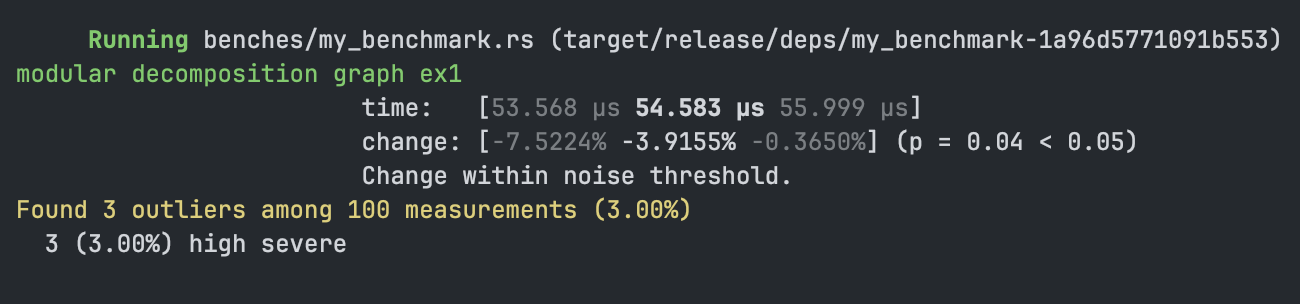
\includegraphics[width=0.80\textwidth]{images/benchmark/benchmark-terminal-output}
                    \caption{Example of Terminal ouput for modular decomposition of graph ex1}
                    \label{fig:example-of-terminal-output}
                \end{figure}
        \item \textbf{HTML Reports:}
        \begin{figure}[!h]
            \centering
            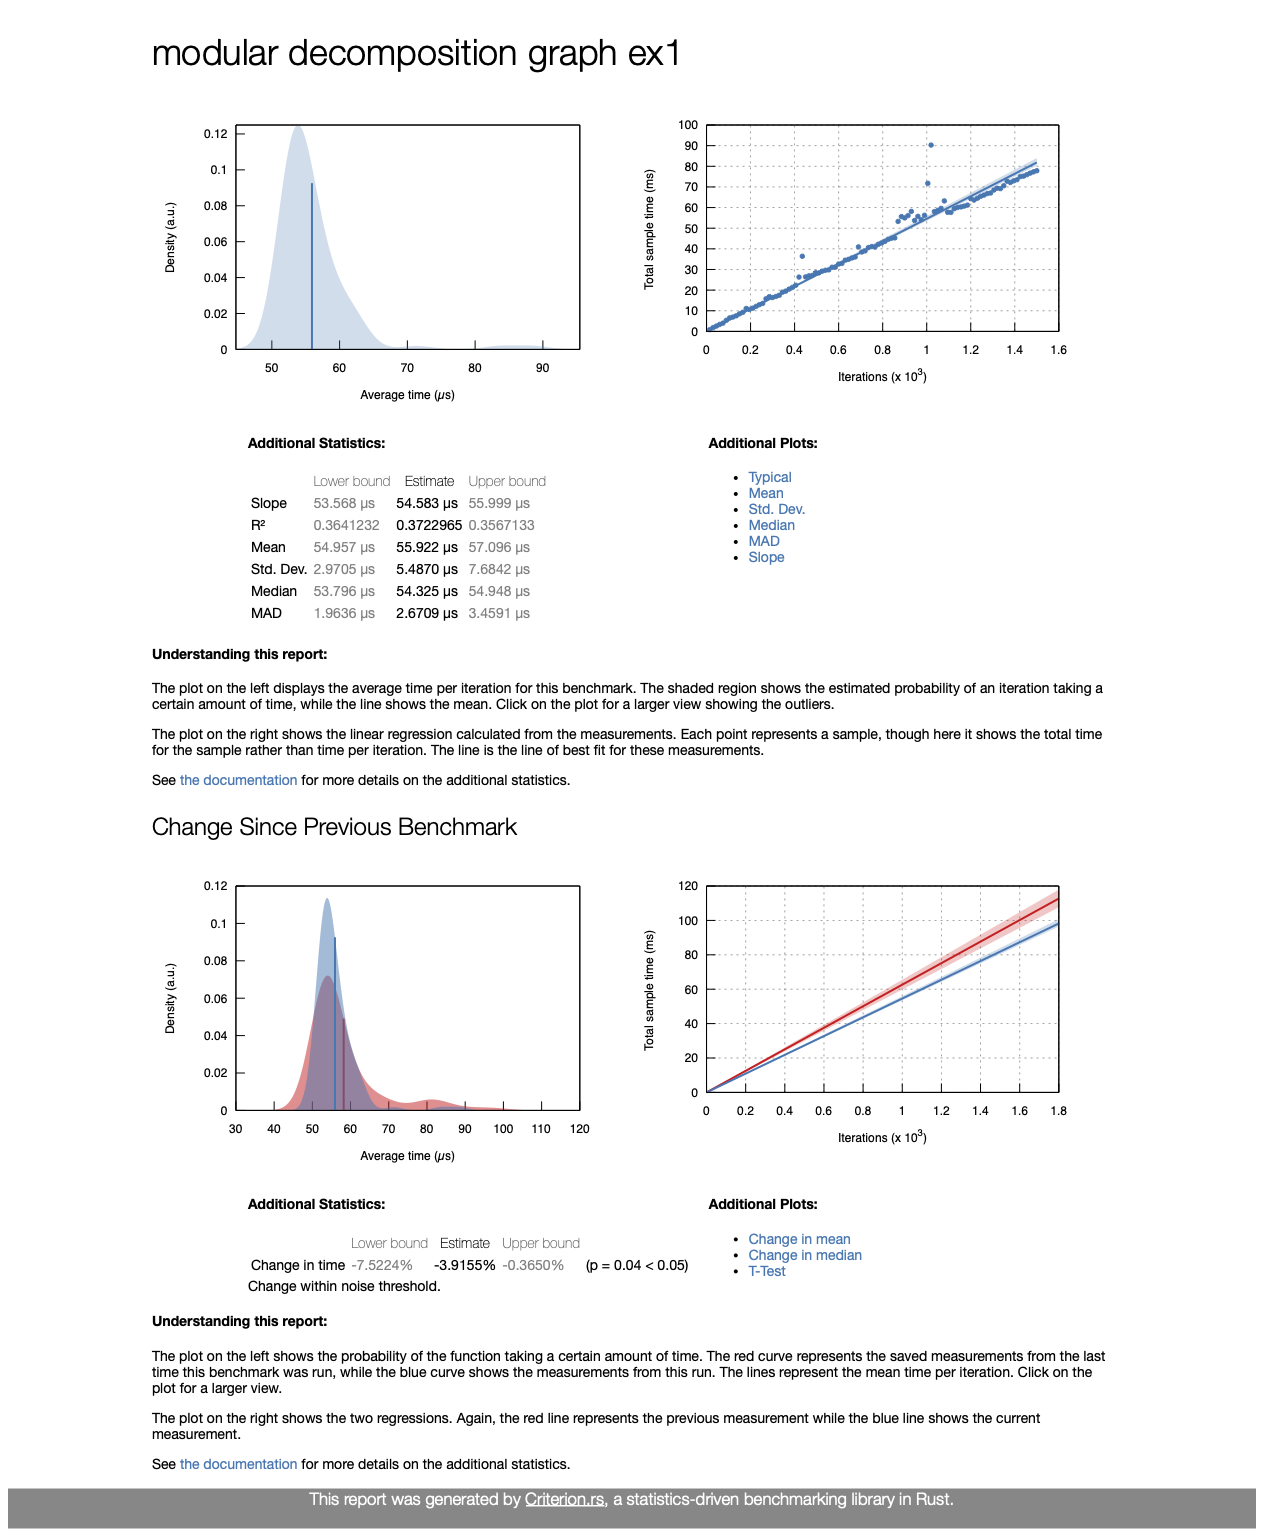
\includegraphics[width=1\textwidth]{images/benchmark/benchmark-html-output}
            \caption{Example of HTML ouput for modular decomposition of graph ex1}
            \label{fig:example-of-html-output}
        \end{figure}
    \end{enumerate}
\end{myex}


For the Python benchmark, I'm going to use the pytest-benchmark\cite{pytestbenchmark} tool to get almost the same execution details as those offered by Rust's Criterion.
While SageMath does not have a benchmarking library as sophisticated as Criterion for Rust, you can still obtain similar performance metrics using Python tools, combined with SageMath.
To replicate the style of results we get from Criterion in Rust, i use the following approach in SageMath:
\begin{itemize}
    \item \textbf{Multiple Timings and Averages:} Run the code multiple times to get an average execution time.
    \item \textbf{Statistical Reporting:} Report min, max, and mean execution times, along with standard deviation, similar to Criterion’s output.
\end{itemize}

\begin{myex}[Example Benchmark Code SageMath]

\end{myex}

\begin{lstlisting}[language=Python, style=python, caption={Example of benchmark code for modular decomposition}, label={lst:sagemath-example-of-benchmark-code}, firstnumber=1]
    import time
    import numpy as np

    def benchmark_modular_decomposition(graph, iterations=100):
        times = []

        for _ in range(iterations):
            # Start timer
            start_time = time.time()

            # Perform the computation
            graph.modular_decomposition()

            # Stop timer
            end_time = time.time()

            # Record execution time in microseconds (µs)
            execution_time = (end_time - start_time)
            times.append(execution_time)

        # Calculate benchmark statistics using NumPy
        min_time = np.min(times)
        max_time = np.max(times)
        mean_time = np.mean(times)
        stdev_time = np.std(times)

        # Print results in seconds (s)
        print(f"Benchmark Results (over {iterations} iterations) in s:")
        print(f"Min Time: {min_time:.2f} s")
        print(f"Max Time: {max_time:.2f} s")
        print(f"Mean Time: {mean_time:.2f} s")
        print(f"Standard Deviation: {stdev_time:.2f} s")
\end{lstlisting}


\section{Result for small graphs : 10 nodes}\label{sec:result-for-small-graphs}

Let's start with the first test on the graph in figure\ref{fig:example-undirected-graph} and in figure\ref{fig:example-directed-graph}.
Here it's called a small graph because of its size, containing just 11 nodes for the first graph and 8 for the second.

\subsection{Benchmark for simple undirected graph\ref{fig:example-undirected-graph}}\label{subsec:benchmark-for-simple-undirected-graph}

\subsubsection*{SageMath Result}

\begin{figure}[!h]
    \centering
    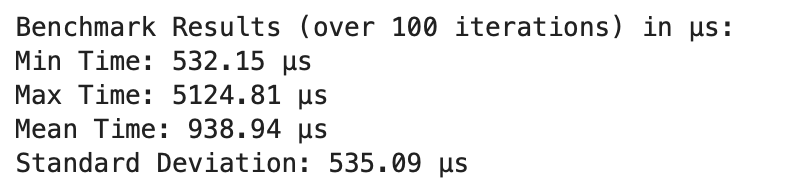
\includegraphics[width=0.60\textwidth]{images/benchmark/graph_wikipedia/benchmark_graph_wikipedia_sagemath}
    \caption{Result benchmark SageMath}
    \label{fig:benchmark-graph-wikipedia-sagemath}
\end{figure}

\subsubsection*{Python Result}
\begin{figure}[!h]
    \centering
    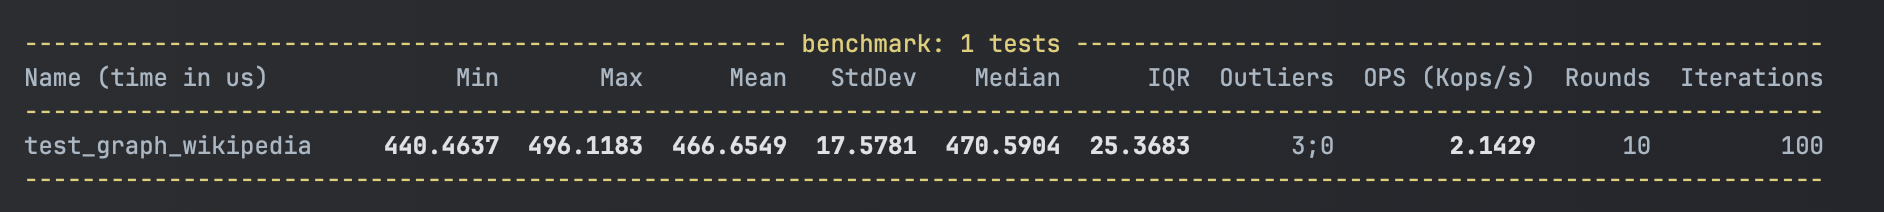
\includegraphics[width=1\textwidth]{images/benchmark/graph_wikipedia/benchmark_graph_wikipedia_python}
    \caption{Result benchmark Python}
    \label{fig:benchmark-graph-wikipedia-python}
\end{figure}

\subsubsection*{Rust Result}
\begin{figure}[!h]
    \centering
    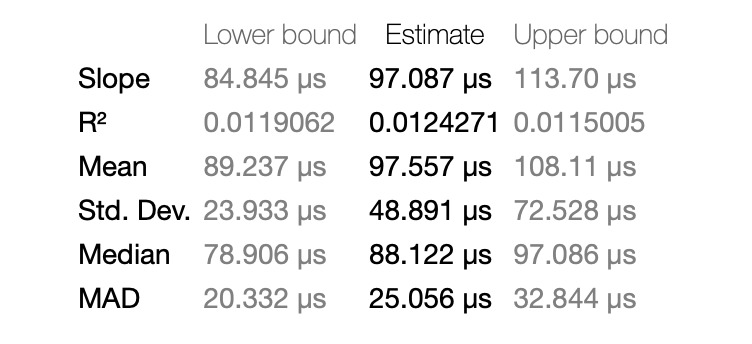
\includegraphics[width=0.60\textwidth]{images/benchmark/graph_wikipedia/benchmark_graph_wikipedia_rust}
    \caption{Result benchmark Python}
    \label{fig:benchmark-graph-wikipedia-rust}
\end{figure}


\subsection{Benchmark for simple directed graph\ref{fig:example-directed-graph}}\label{subsec:benchmark-for-simple-directed-graph}

\subsubsection*{SageMath Result}
\begin{figure}[!h]
    \centering
    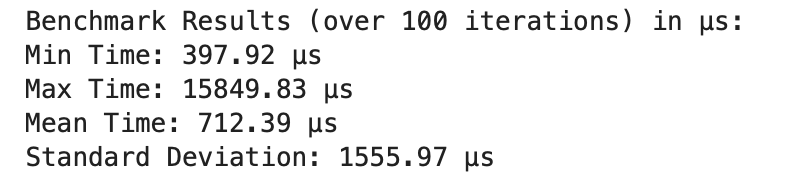
\includegraphics[width=0.60\textwidth]{images/benchmark/digraph/benchmark_digraph_sagemath}
    \caption{Result benchmark SageMath}
    \label{fig:benchmark-digraph-sagemath}
\end{figure}

\subsubsection*{Python Result}
\begin{figure}[!h]
    \centering
    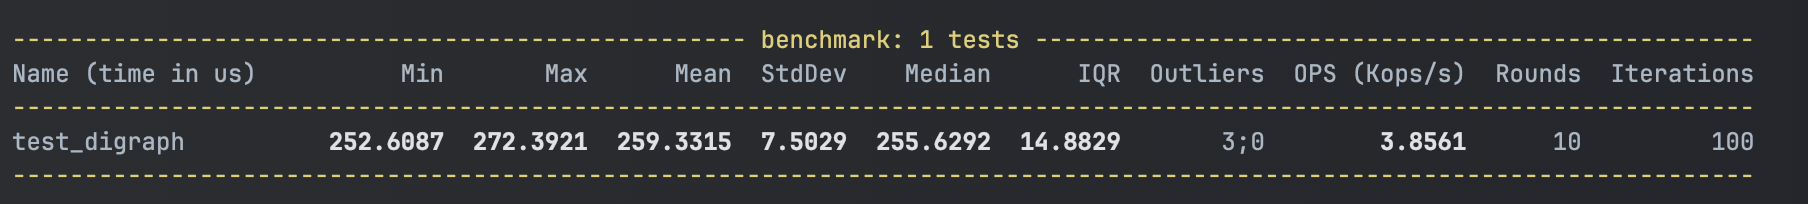
\includegraphics[width=1\textwidth]{images/benchmark/digraph/benchmark_digraph_python}
    \caption{Result benchmark Python}
    \label{fig:benchmark-digraph-python}
\end{figure}

\subsubsection*{Rust Result}
\begin{figure}[!h]
    \centering
    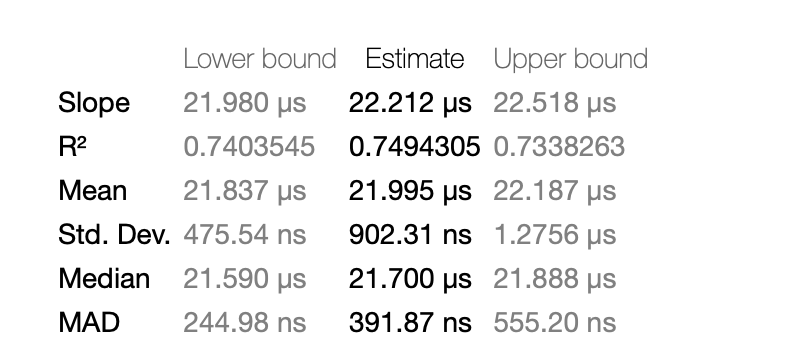
\includegraphics[width=0.60\textwidth]{images/benchmark/digraph/benchmark_digraph_rust}
    \caption{Result benchmark Python}
    \label{fig:benchmark-digraph-rust}
\end{figure}


\section{Result for large graphs : 100 nodes}\label{sec:result-for-large-graphs}

\subsubsection*{SageMath Result}
\begin{figure}[!h]
    \centering
    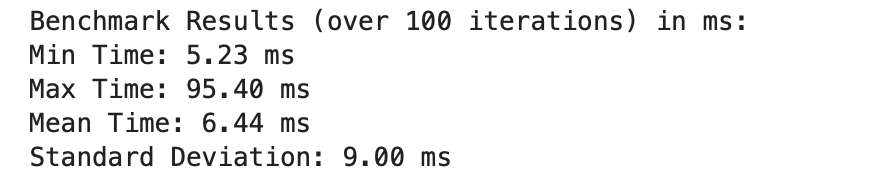
\includegraphics[width=0.60\textwidth]{images/benchmark/large_graph/benchmark_large_graph_sagemath}
    \caption{Result benchmark SageMath}
    \label{fig:benchmark-large-graph-sagemath}
\end{figure}

\subsubsection*{Python Result}
\begin{figure}[!h]
    \centering
    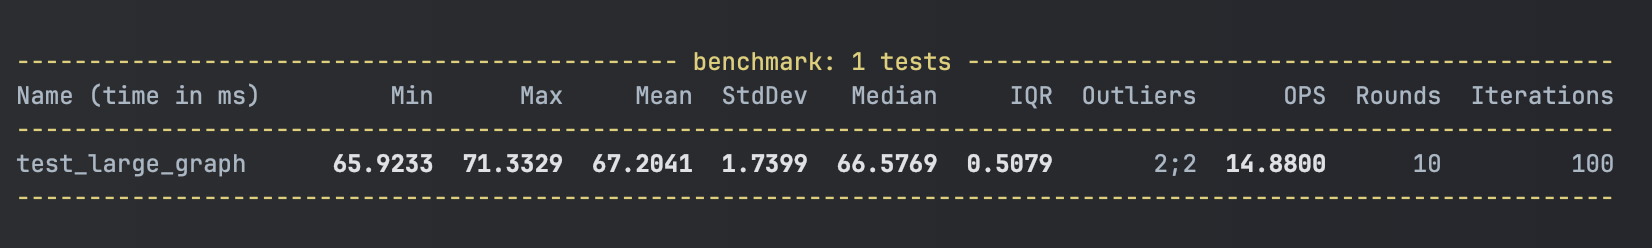
\includegraphics[width=1\textwidth]{images/benchmark/large_graph/benchmark_large_graph_python}
    \caption{Result benchmark Python}
    \label{fig:benchmark-large-graph-python}
\end{figure}

\subsubsection*{Rust Result}
\begin{figure}[!h]
    \centering
    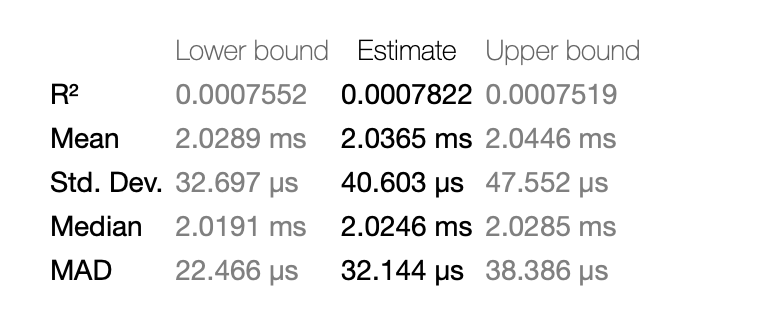
\includegraphics[width=0.60\textwidth]{images/benchmark/large_graph/benchmark_large_graph_rust}
    \caption{Result benchmark Python}
    \label{fig:benchmark-large-graph-rust}
\end{figure}


\section{Result for Too Large graphs : 500 nodes}\label{sec:result-for-too-large-graphs}

\subsubsection*{SageMath Result}
\begin{figure}[!h]
    \centering
    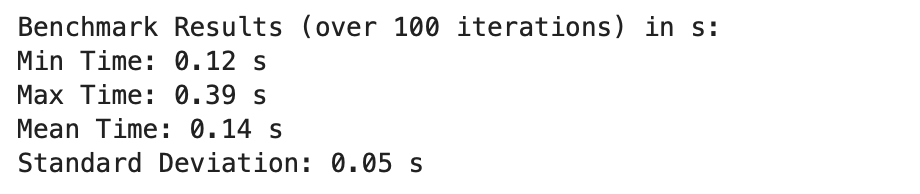
\includegraphics[width=0.60\textwidth]{images/benchmark/too_large_graph/benchmark_too_large_graph_sagemath}
    \caption{Result benchmark SageMath}
    \label{fig:benchmark-too-large-graph-sagemath}
\end{figure}

\subsubsection*{Python Result}
\begin{figure}[!h]
    \centering
    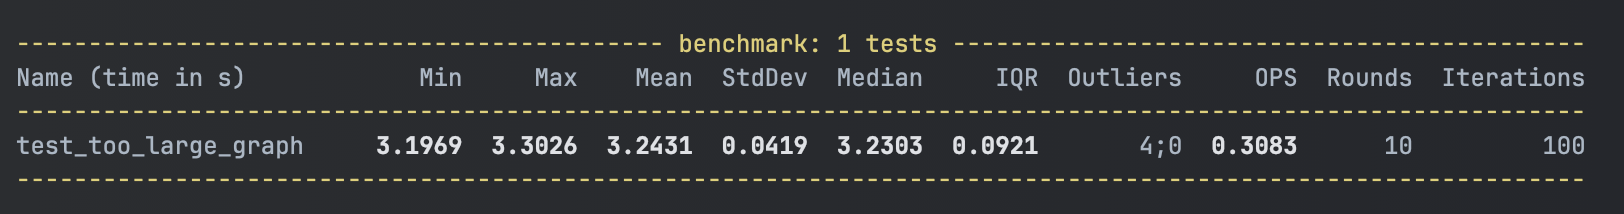
\includegraphics[width=1\textwidth]{images/benchmark/too_large_graph/benchmark_too_large_graph_python}
    \caption{Result benchmark Python}
    \label{fig:benchmark-too-large-graph-python}
\end{figure}

\subsubsection*{Rust Result}
\begin{figure}[!h]
    \centering
    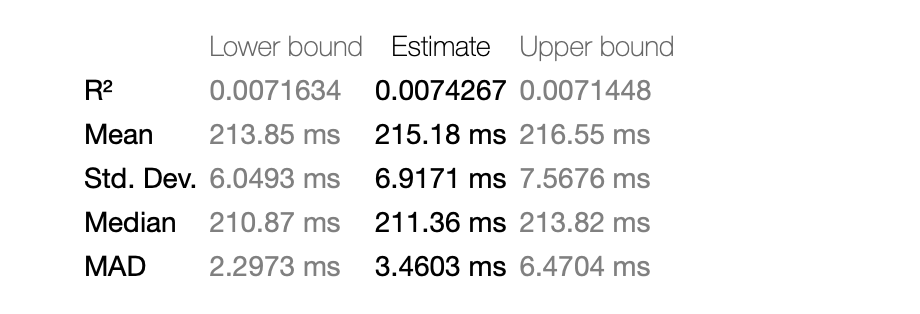
\includegraphics[width=0.60\textwidth]{images/benchmark/too_large_graph/benchmark_too_large_graph_rust}
    \caption{Result benchmark Python}
    \label{fig:benchmark-too-large-graph-rust}
\end{figure}


\section{Conclusion}\label{sec:conclusion}

From these results, we can clearly see that the performance in terms of execution speed of the Rust version is decidedly better, with a very considerable gap compared with the improvement in the SageMath version and Python.




% Conclusion
    %! Author = adrien koumgang tegantchouang
%! Date = 09/07/24


\chapter{Conclusion}\label{ch:conclusion}




    \bibliographystyle{IEEEtran}
    \bibliography{bibliography}
    % \printbibliography


% acknowledgement
    

\chapter*{Acknowledgments}\label{ch:acknowledgments}

I would like to express my deepest gratitude to all those who have supported me throughout the process of writing this thesis.
First and foremost, I am incredibly grateful to my external supervisors, Prof. Frédéric Peschanshi and Prof. Antoine Genitrini,
whose guidance, expertise, and encouragement were invaluable at every stage of this research.
Their insights into graph theory and algorithm design provided me with the foundation I needed to explore modular decomposition in depth.

A special thanks goes to my internal supervisor, Prof. Andrea Corradini, for his constant support, constructive feedback, and mentorship throughout the development of the thesis.
His attention to detail and dedication to excellence inspired me to push the boundaries of my work and ensure that the research met the highest standards.

I would also like to thank the entire Computer Science department, which provided me with the courses and environment I needed to acquire the knowledge I now possess, and which greatly contributed to the completion of this work.

Again, I would also like to thank Eleni Pistiloglou, whose prior work on modular decomposition laid the groundwork for my own contributions.

I am immensely grateful to my family and friends for their unwavering support and encouragement, especially during the more challenging moments of this journey.
Their belief in me has been a constant source of motivation.
Even when they're far away from me, from another continent, they're all close to me.

A special thought to my family from another parent, my brothers and sisters from another father and another mother, as we say so well in Cameroon,
to Amira, Arnold, Christelle, Lorenza, Maria, Martina, Mimie des Mimie (whose smile gave me lots of energy, ahahahah), Pavel, Rhynelle, Ulrich, Yannick,
who throughout this work have motivated me to keep moving forward.
They have been there for me both physically and psychologically, encouraging me to believe in myself, in my abilities and in my dream.

I'd like to thank all those people who have had an impact on my life and contributed, in one way or another, to bringing me to where I am today.
A special thought to my colleagues and bosses at IperDesign (Newton) who supported me and gave me the time I needed to write this report.
I think of Andrea, Eliana, Flavia, Martina, Mattia, and Nicola.

I am also thankful to JetBrains for offering the tools such as RustRover, which significantly aided the development and testing of my Rust implementations.

Lastly, I would like to acknowledge the Rust and C++ communities for their contributions to open-source libraries and documentation, which greatly facilitated my learning and development process.
This work would not have been possible without the collaborative spirit of the open-source community.

I dedicate my thesis to my second mother, Maman Mireille, who passed away while I was working on this thesis.
We made promises to each other when I left Cameroon, but I won't be able to keep them all, but I'll fight to keep the ones I can.
You who today are in heaven watching over us, know that my love for you remains, your child.




    \include{glossary}

\end{document}
